\subsection{فعالیت برخاستن از زمین}

هدف از بررسی این فعالیت، ارزیابی توانایی سامانه در تفکیک سه سطح عملکردی شبیه‌سازی‌شده در یک حرکت چندمرحله‌ای و نسبتاً پیچیده است. برخاستن از زمین شامل انتقال بدن از وضعیت قرارگرفته روی زمین به حالت ایستاده است و اجرای آن به هماهنگی اندام‌های فوقانی، اندام‌های تحتانی و تنه نیاز دارد. در این بخش، تمرکز تحلیل بر ساختار فضای ویژگی، اثر کاهش بعد و عملکرد مدل‌های مختلف در طبقه‌بندی سطوح عملکردی قرار گرفته است.

\subsubsection{گزارش کلی فعالیت}

فعالیت برخاستن از زمین، برخلاف فعالیت ایستادن، دارای چند مرحله حرکتی مشخص است. این مراحل شامل آغاز حرکت از سطح زمین، تغییر وضعیت تنه، انتقال وزن، استفاده احتمالی از دست‌ها یا زانوها برای ایجاد تکیه‌گاه، بلندشدن و در نهایت رسیدن به وضعیت ایستاده پایدار هستند.

برای پیش‌پردازش اولیه داده‌ها از فیلتر استفاده شد تا نویزهای موجود در سیگنال حسگرها کاهش یابد. همچنین با توجه به وجود بازه‌های بدون حرکت در ابتدا و انتهای آزمون، جداسازی بازه اصلی فعالیت می‌تواند باعث شود ویژگی‌ها بیشتر تحت تأثیر بخش واقعی حرکت قرار گیرند.

\textbf{TODO: مشخص شود که نتایج نهایی این فعالیت بر اساس داده‌های بدون جداسازی فعالیت، داده‌های جداسازی‌شده یا مقایسه هر دو حالت گزارش شده‌اند.}

نمونه سیگنال در
\autoref{fig:Sit_To_Stand_normal_signal_sample}
نشان می‌دهد که فعالیت برخاستن از زمین دارای تغییرات قابل‌توجهی در شتاب و سرعت زاویه‌ای حسگرها است. این تغییرات به دلیل جابه‌جایی هم‌زمان تنه و اندام‌ها و عبور از چند وضعیت بدنی متفاوت ایجاد می‌شوند.

انتظار می‌رود حسگر نصب‌شده روی سر تغییر وضعیت کلی تنه و انتقال بدن به حالت قائم را نشان دهد. حسگرهای نصب‌شده روی پاها نیز اطلاعات مربوط به انتقال وزن، قرارگیری پاها و مرحله نهایی برخاستن را ثبت می‌کنند. در صورت استفاده از دست‌ها برای ایجاد تکیه‌گاه، سیگنال حسگرهای دست می‌تواند تغییرات بزرگ‌تری داشته باشد. بنابراین، نحوه مشارکت اندام‌های مختلف یکی از عوامل مهم در تفکیک سطوح عملکردی این فعالیت است.

\textbf{TODO: بر اساس شکل سیگنال مشخص شود که بیشترین تغییرات مربوط به کدام حسگرها و کدام محورها بوده است. همچنین وجود قله‌های مشخص، اختلاف مدت اجرای حرکت یا تفاوت دامنه سیگنال میان طبقه‌ها گزارش شود.}

\begin{figure}[H]
	\centering
	
\includegraphics[width=0.80\linewidth]{Images/Generated/TaskResults/Sit_To_Stand/Normal/signal_sample.png}
	\caption{نمونه سیگنال‌های ثبت‌شده در فعالیت برخاستن از زمین}
	\label{fig:Sit_To_Stand_normal_signal_sample}
\end{figure}

در این فعالیت، توزیع نمونه‌ها میان سه طبقه یکسان در نظر گرفته شد. از آنجا که ایجاد داده‌های حرکتی شبیه‌سازی‌شده نیز بخشی از روند پژوهش بود، برای هر سه سطح عملکردی تعداد یکسانی آزمون انجام شد تا اثر نامتوازن‌بودن تعداد طبقه‌ها بر آموزش و ارزیابی مدل‌ها کاهش یابد.

\subsubsection{ساختار ویژگی‌ها}

در فعالیت برخاستن از زمین، تعداد ویژگی‌های استخراج‌شده نسبت به تعداد نمونه‌ها زیاد بود؛ بنابراین ساختار همبستگی میان ویژگی‌ها بررسی شد. نقشه همبستگی در
\autoref{fig:Sit_To_Stand_normal_feature_correlation}
ارتباط میان تعدادی از ویژگی‌های استخراج‌شده از حسگرها و محورهای مختلف را نشان می‌دهد.

با توجه به ماهیت دینامیکی این فعالیت، انتظار می‌رود ویژگی‌هایی مانند انرژی، دامنه تغییرات، انحراف معیار، ریشه میانگین مربعات و مقادیر بیشینه در برخی حسگرها رفتار مشابهی داشته باشند. همچنین ویژگی‌های مربوط به حسگرهای دو سمت بدن ممکن است به دلیل مشارکت هم‌زمان اندام‌ها با یکدیگر همبستگی داشته باشند.

\textbf{TODO: بر اساس نقشه همبستگی مشخص شود که همبستگی شدید بیشتر میان چه ویژگی‌ها، حسگرها یا محورهایی مشاهده شده است.}

\begin{figure}[H]
	\centering
	
\includegraphics[width=0.75\linewidth]{Images/Generated/TaskResults/Sit_To_Stand/Normal/feature_correlation_heatmap.png}
	\caption{نقشه همبستگی ویژگی‌های منتخب در فعالیت برخاستن از زمین}
	\label{fig:Sit_To_Stand_normal_feature_correlation}
\end{figure}

اگرچه استفاده از تمام ویژگی‌های استخراج‌شده ممکن است به عملکرد مناسب طبقه‌بند منجر شود، تعداد زیاد ویژگی‌ها در مقایسه با تعداد نمونه‌ها می‌تواند احتمال بیش‌برازش را افزایش دهد. علاوه بر این، وجود ویژگی‌های همبسته موجب می‌شود بخشی از اطلاعات ورودی تکراری باشد. به همین دلیل، در ادامه کاهش بعد فضای ویژگی‌ها مورد بررسی قرار گرفت.

\subsubsection{کاهش بعد ویژگی‌ها}
\label{sec:dimension_reduction_Sit_To_Stand}

همان‌طور که در
\autoref{sec:demansionreduction}
اشاره شد، از تحلیل مؤلفه‌های اصلی برای کاهش بعد ویژگی‌ها استفاده شد. در فعالیت برخاستن از زمین، با استفاده از
\textbf{TODO: تعداد مؤلفه اصلی}
توانستیم ۹۵ درصد واریانس داده‌های اولیه را حفظ کنیم.

طبق نمودار واریانس تجمعی در
\autoref{fig:Sit_To_Stand_normal_pca_variance}،
بخش قابل‌توجهی از تغییرات داده‌ها توسط مؤلفه‌های ابتدایی نمایش داده می‌شود. این موضوع نشان می‌دهد که اطلاعات موجود در ویژگی‌های اولیه را می‌توان با تعداد کمتری متغیر جدید خلاصه کرد.

برای مثال، با استفاده از
\textbf{TODO: تعداد مؤلفه اول}
می‌توان حدود
\textbf{TODO: درصد واریانس}
از واریانس داده‌ها را حفظ کرد. اضافه‌کردن
\textbf{TODO: تعداد مؤلفه‌های بعدی}
تنها موجب افزایش
\textbf{TODO: درصد افزایش واریانس}
در واریانس تجمعی می‌شود. بنابراین، استفاده از تمام مؤلفه‌های لازم برای رسیدن به آستانه ۹۵ درصد لزوماً بهترین انتخاب برای مدل نهایی نیست.

\begin{figure}[H]
	\centering
	
\includegraphics[width=0.8\linewidth]{Images/Generated/TaskResults/Sit_To_Stand/Normal/pca_variance_curve.png}
	\caption{واریانس توضیح‌داده‌شده و واریانس تجمعی مؤلفه‌های اصلی در فعالیت برخاستن از زمین}
	\label{fig:Sit_To_Stand_normal_pca_variance}
\end{figure}

پراکندگی داده‌ها در فضای دو مؤلفه اصلی اول در
\autoref{fig:Sit_To_Stand_normal_pca_scatter}
برای بررسی اولیه ساختار طبقه‌ها نمایش داده شده است. با توجه به چندمرحله‌ای‌بودن برخاستن از زمین، ممکن است بخشی از تفاوت طبقه‌ها در دو مؤلفه نخست دیده شود، اما احتمال هم‌پوشانی نمونه‌ها نیز وجود دارد؛ زیرا افراد می‌توانند برای رسیدن به یک سطح عملکردی از الگوهای حرکتی متفاوتی استفاده کنند.

\textbf{TODO: بر اساس نمودار مشخص شود که آیا سه طبقه جدایی مناسبی دارند، کدام طبقه‌ها بیشتر هم‌پوشانی دارند و آیا نمونه دورافتاده‌ای مشاهده می‌شود.}

\begin{figure}[H]
	\centering
	
\includegraphics[width=0.8\linewidth]{Images/Generated/TaskResults/Sit_To_Stand/Normal/pca_scatter_pc1_pc2.png}
	\caption{پراکندگی نمونه‌های فعالیت برخاستن از زمین در فضای دو مؤلفه اصلی اول}
	\label{fig:Sit_To_Stand_normal_pca_scatter}
\end{figure}

نمودار پراکندگی دو مؤلفه نخست به‌تنهایی برای تصمیم‌گیری درباره قابلیت تفکیک طبقه‌ها کافی نیست؛ زیرا بخشی از اطلاعات ممکن است در مؤلفه‌های بعدی قرار داشته باشد. نتیجه مهم این بخش آن است که استفاده مستقیم از تمام ویژگی‌های اولیه ضروری نیست و می‌توان فضای ورودی مدل را با حفظ بخش اصلی اطلاعات کاهش داد.

\subsubsection{عملکرد طبقه‌بندها}

عملکرد سه طبقه‌بند ماشین بردار پشتیبان، K-نزدیک‌ترین همسایه و جنگل تصادفی در
\autoref{fig:Sit_To_Stand_accuracy_bar_baseline}
مقایسه شده است. معیار اولیه در این مقایسه دقت طبقه‌بندی بود.

\textbf{TODO: نام مدل دارای بیشترین دقت و مقدار تقریبی دقت آن بر اساس نمودار نوشته شود. همچنین مشخص شود اختلاف مدل‌ها قابل‌توجه بوده است یا خیر.}

\begin{figure}[H]
	\centering
	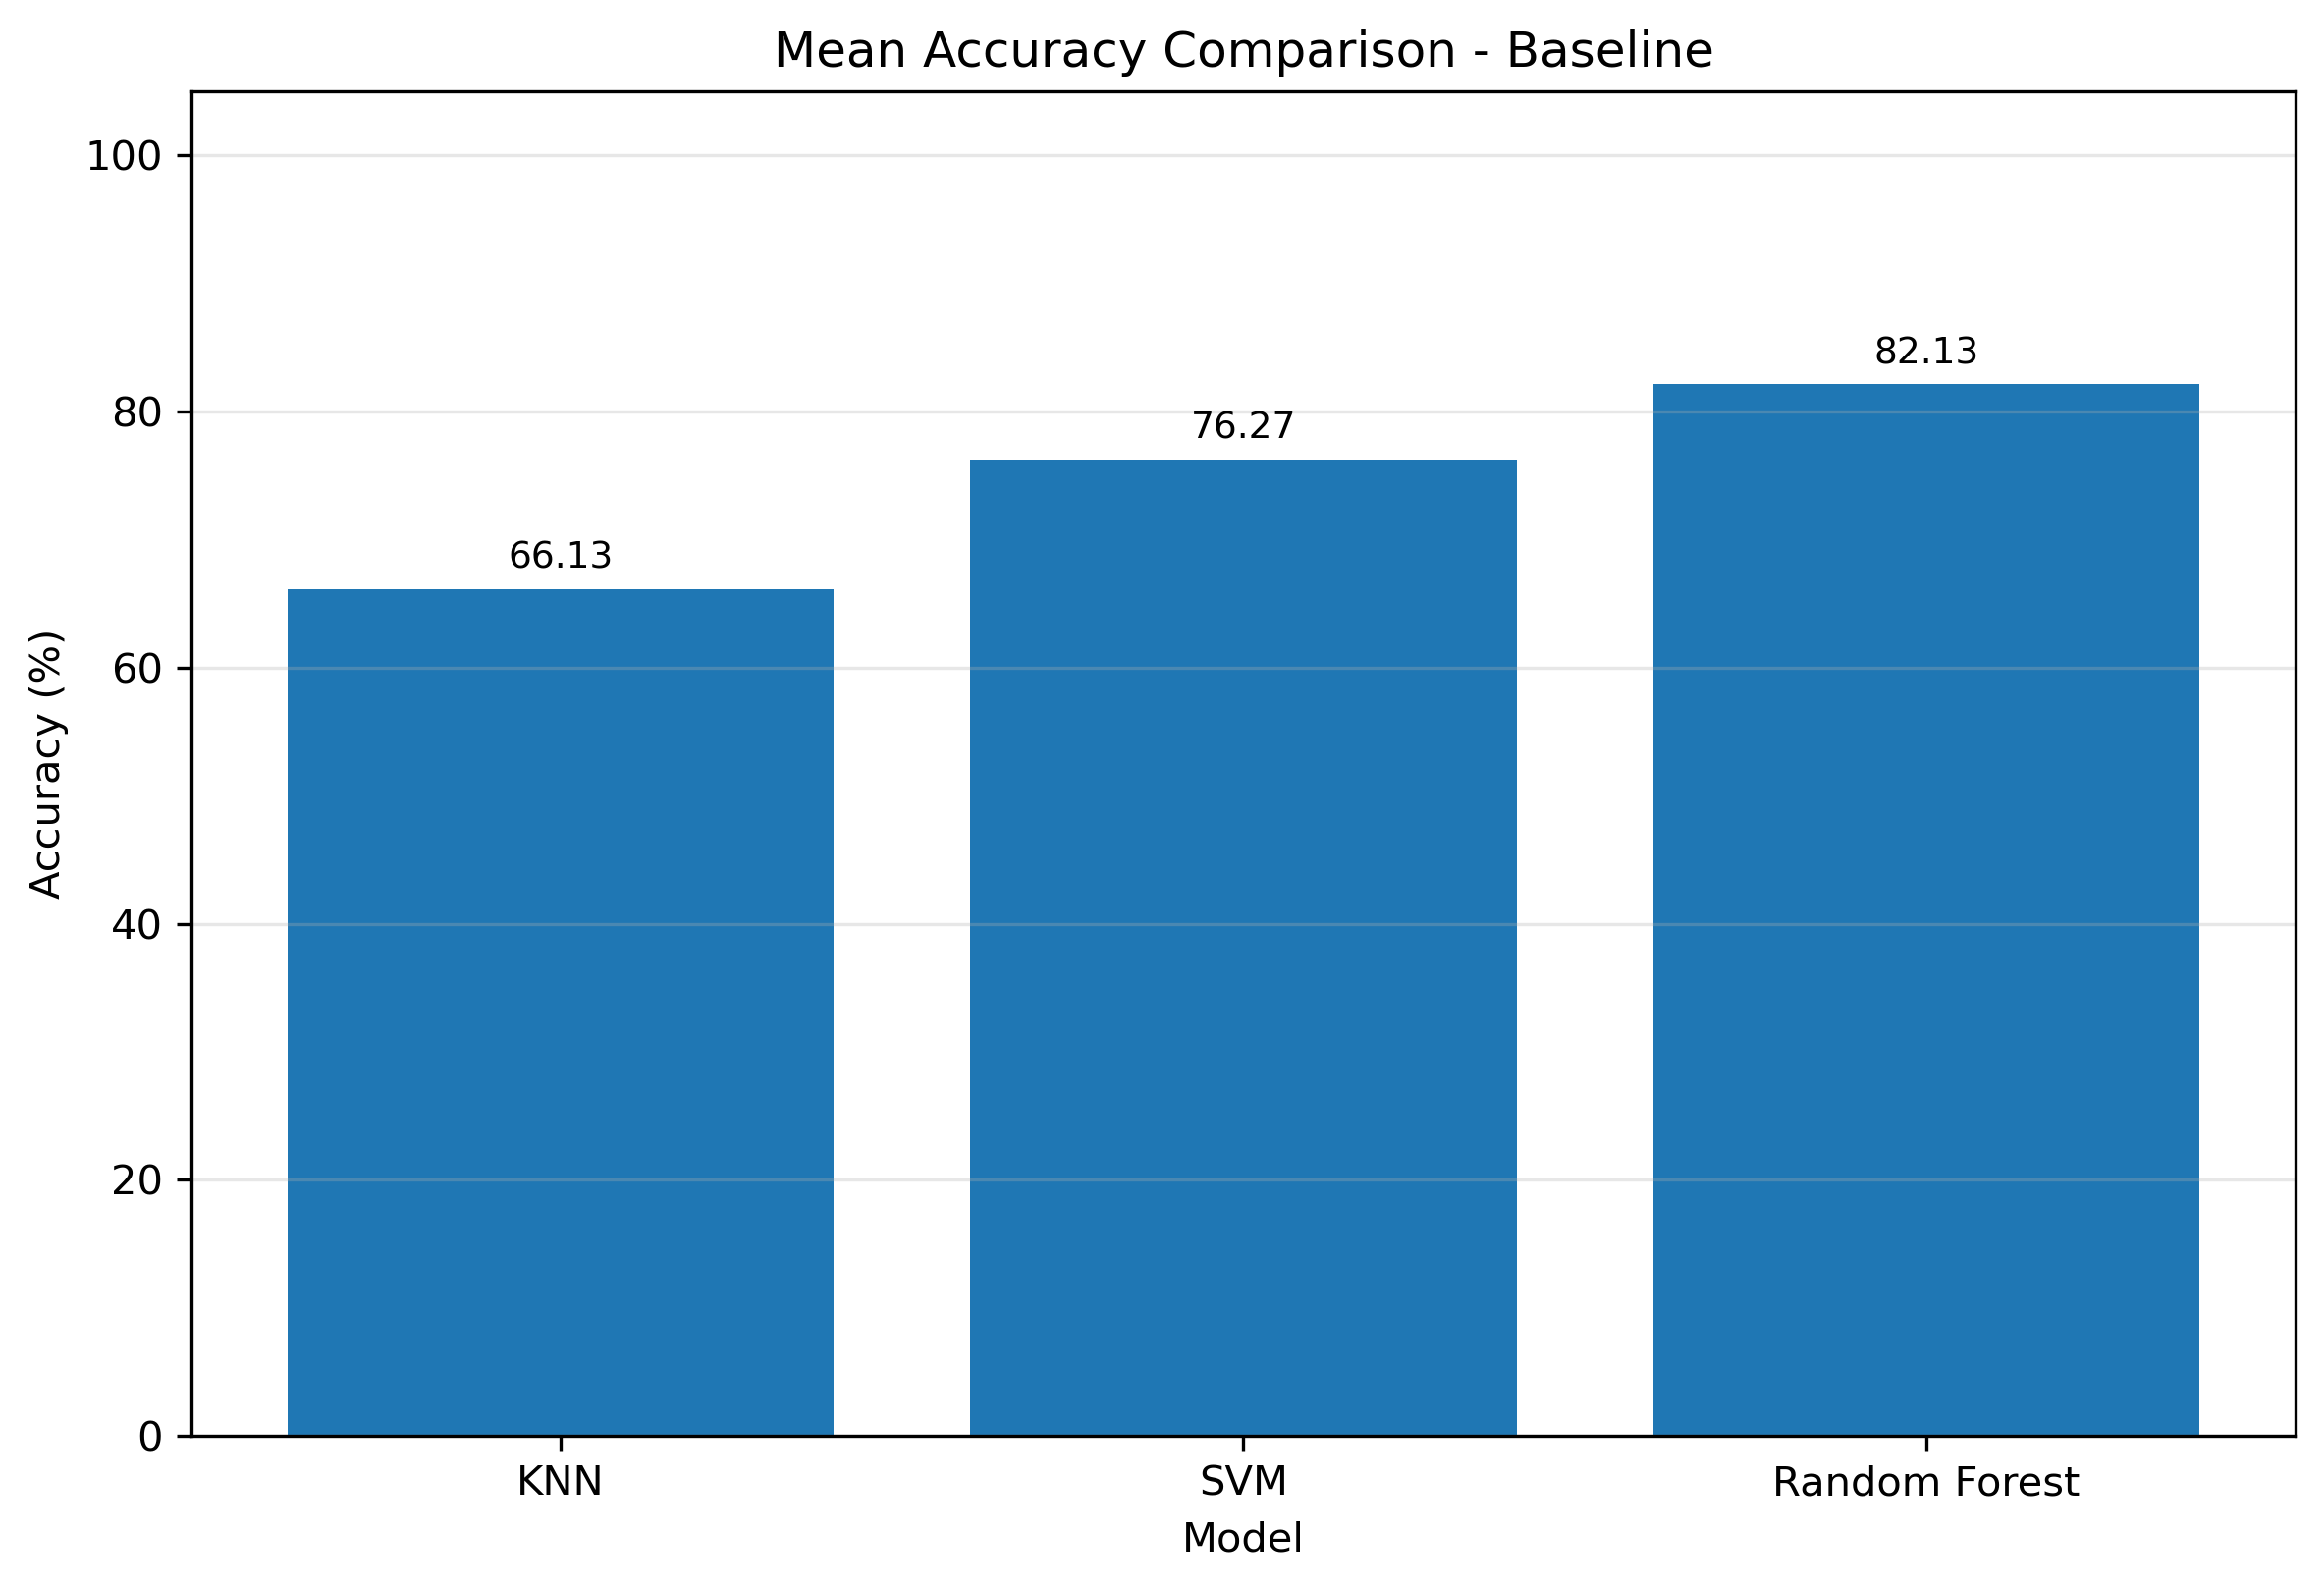
\includegraphics[width=0.8\linewidth]{../Results/Sit_To_Stand/Baseline/Accuracy_Bar_Baseline}
	\caption{مقایسه عملکرد مدل‌ها بر اساس دقت در فعالیت برخاستن از زمین}
	\label{fig:Sit_To_Stand_accuracy_bar_baseline}
\end{figure}

از آنجا که دقت به‌تنهایی نمی‌تواند تمام جنبه‌های عملکرد مدل را نشان دهد، توزیع معیارهای دقت، صحت، بازخوانی و امتیاز F1 نیز در
\autoref{fig:Sit_To_Stand_metric_distribution_baseline}
بررسی شد.

\textbf{TODO: بر اساس نمودار مشخص شود کدام مدل بالاترین میانگین و کدام مدل کمترین پراکندگی را داشته است. در صورت تفاوت میان برتری مدل‌ها در معیارهای مختلف، این موضوع توضیح داده شود.}

\begin{figure}[H]
	\centering
	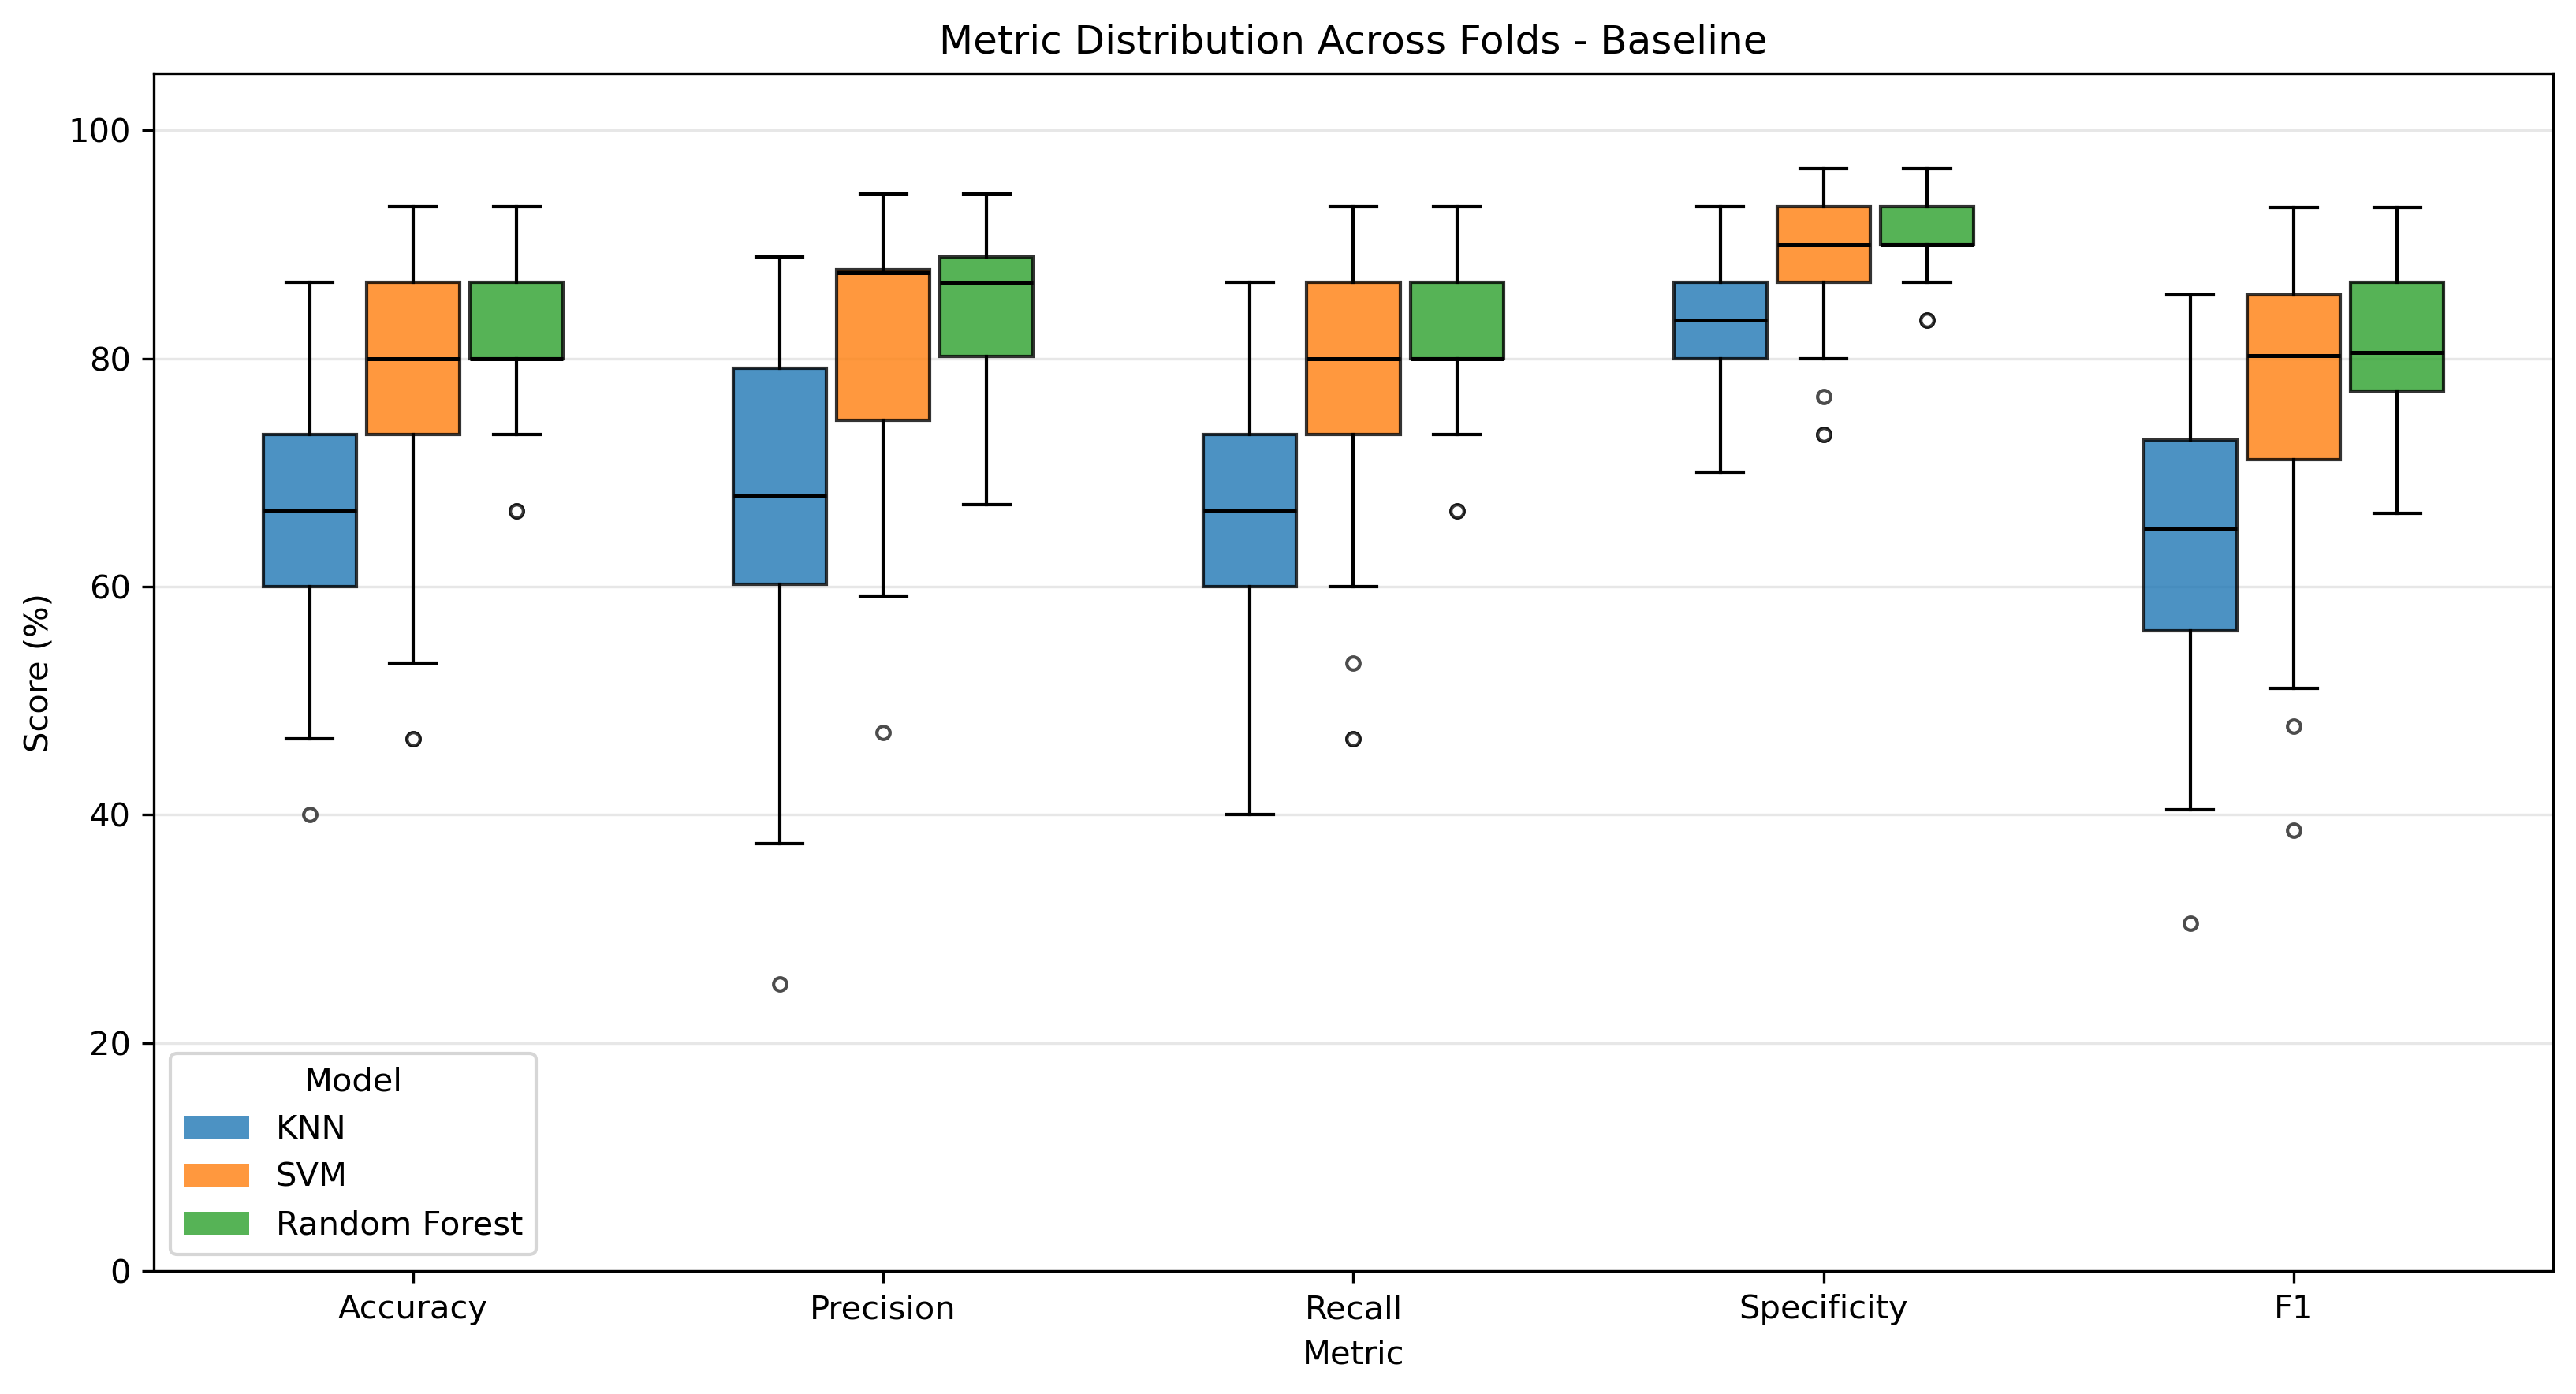
\includegraphics[width=0.8\linewidth]{../Results/Sit_To_Stand/Baseline/Metric_Distribution_Baseline}
	\caption{مقایسه توزیع معیارهای ارزیابی مدل‌ها در فعالیت برخاستن از زمین}
	\label{fig:Sit_To_Stand_metric_distribution_baseline}
\end{figure}

پراکندگی معیارها در تقسیم‌بندی‌های مختلف
\footnote{\lr{Fold}}
برای بررسی ثبات مدل‌ها استفاده شد. مدلی که علاوه بر میانگین عملکرد بالا، پراکندگی کمتری داشته باشد، وابستگی کمتری به نحوه تقسیم داده‌ها خواهد داشت و گزینه مطمئن‌تری برای انتخاب نهایی محسوب می‌شود.

طبق موارد مطرح‌شده در
\autoref{sec:dimension_reduction_Sit_To_Stand}،
عملکرد مدل‌ها پس از اعمال تحلیل مؤلفه‌های اصلی نیز بررسی شد. نتایج این حالت در
\autoref{fig:Sit_To_Stand_metric_distribution_pipeline_pca}
ارائه شده‌اند.

\textbf{TODO: مدل یا مدل‌های برتر پس از اعمال PCA مشخص شوند و توضیح داده شود که کاهش بعد موجب بهبود، کاهش یا ثابت‌ماندن عملکرد هر مدل شده است.}

\begin{figure}[H]
	\centering
	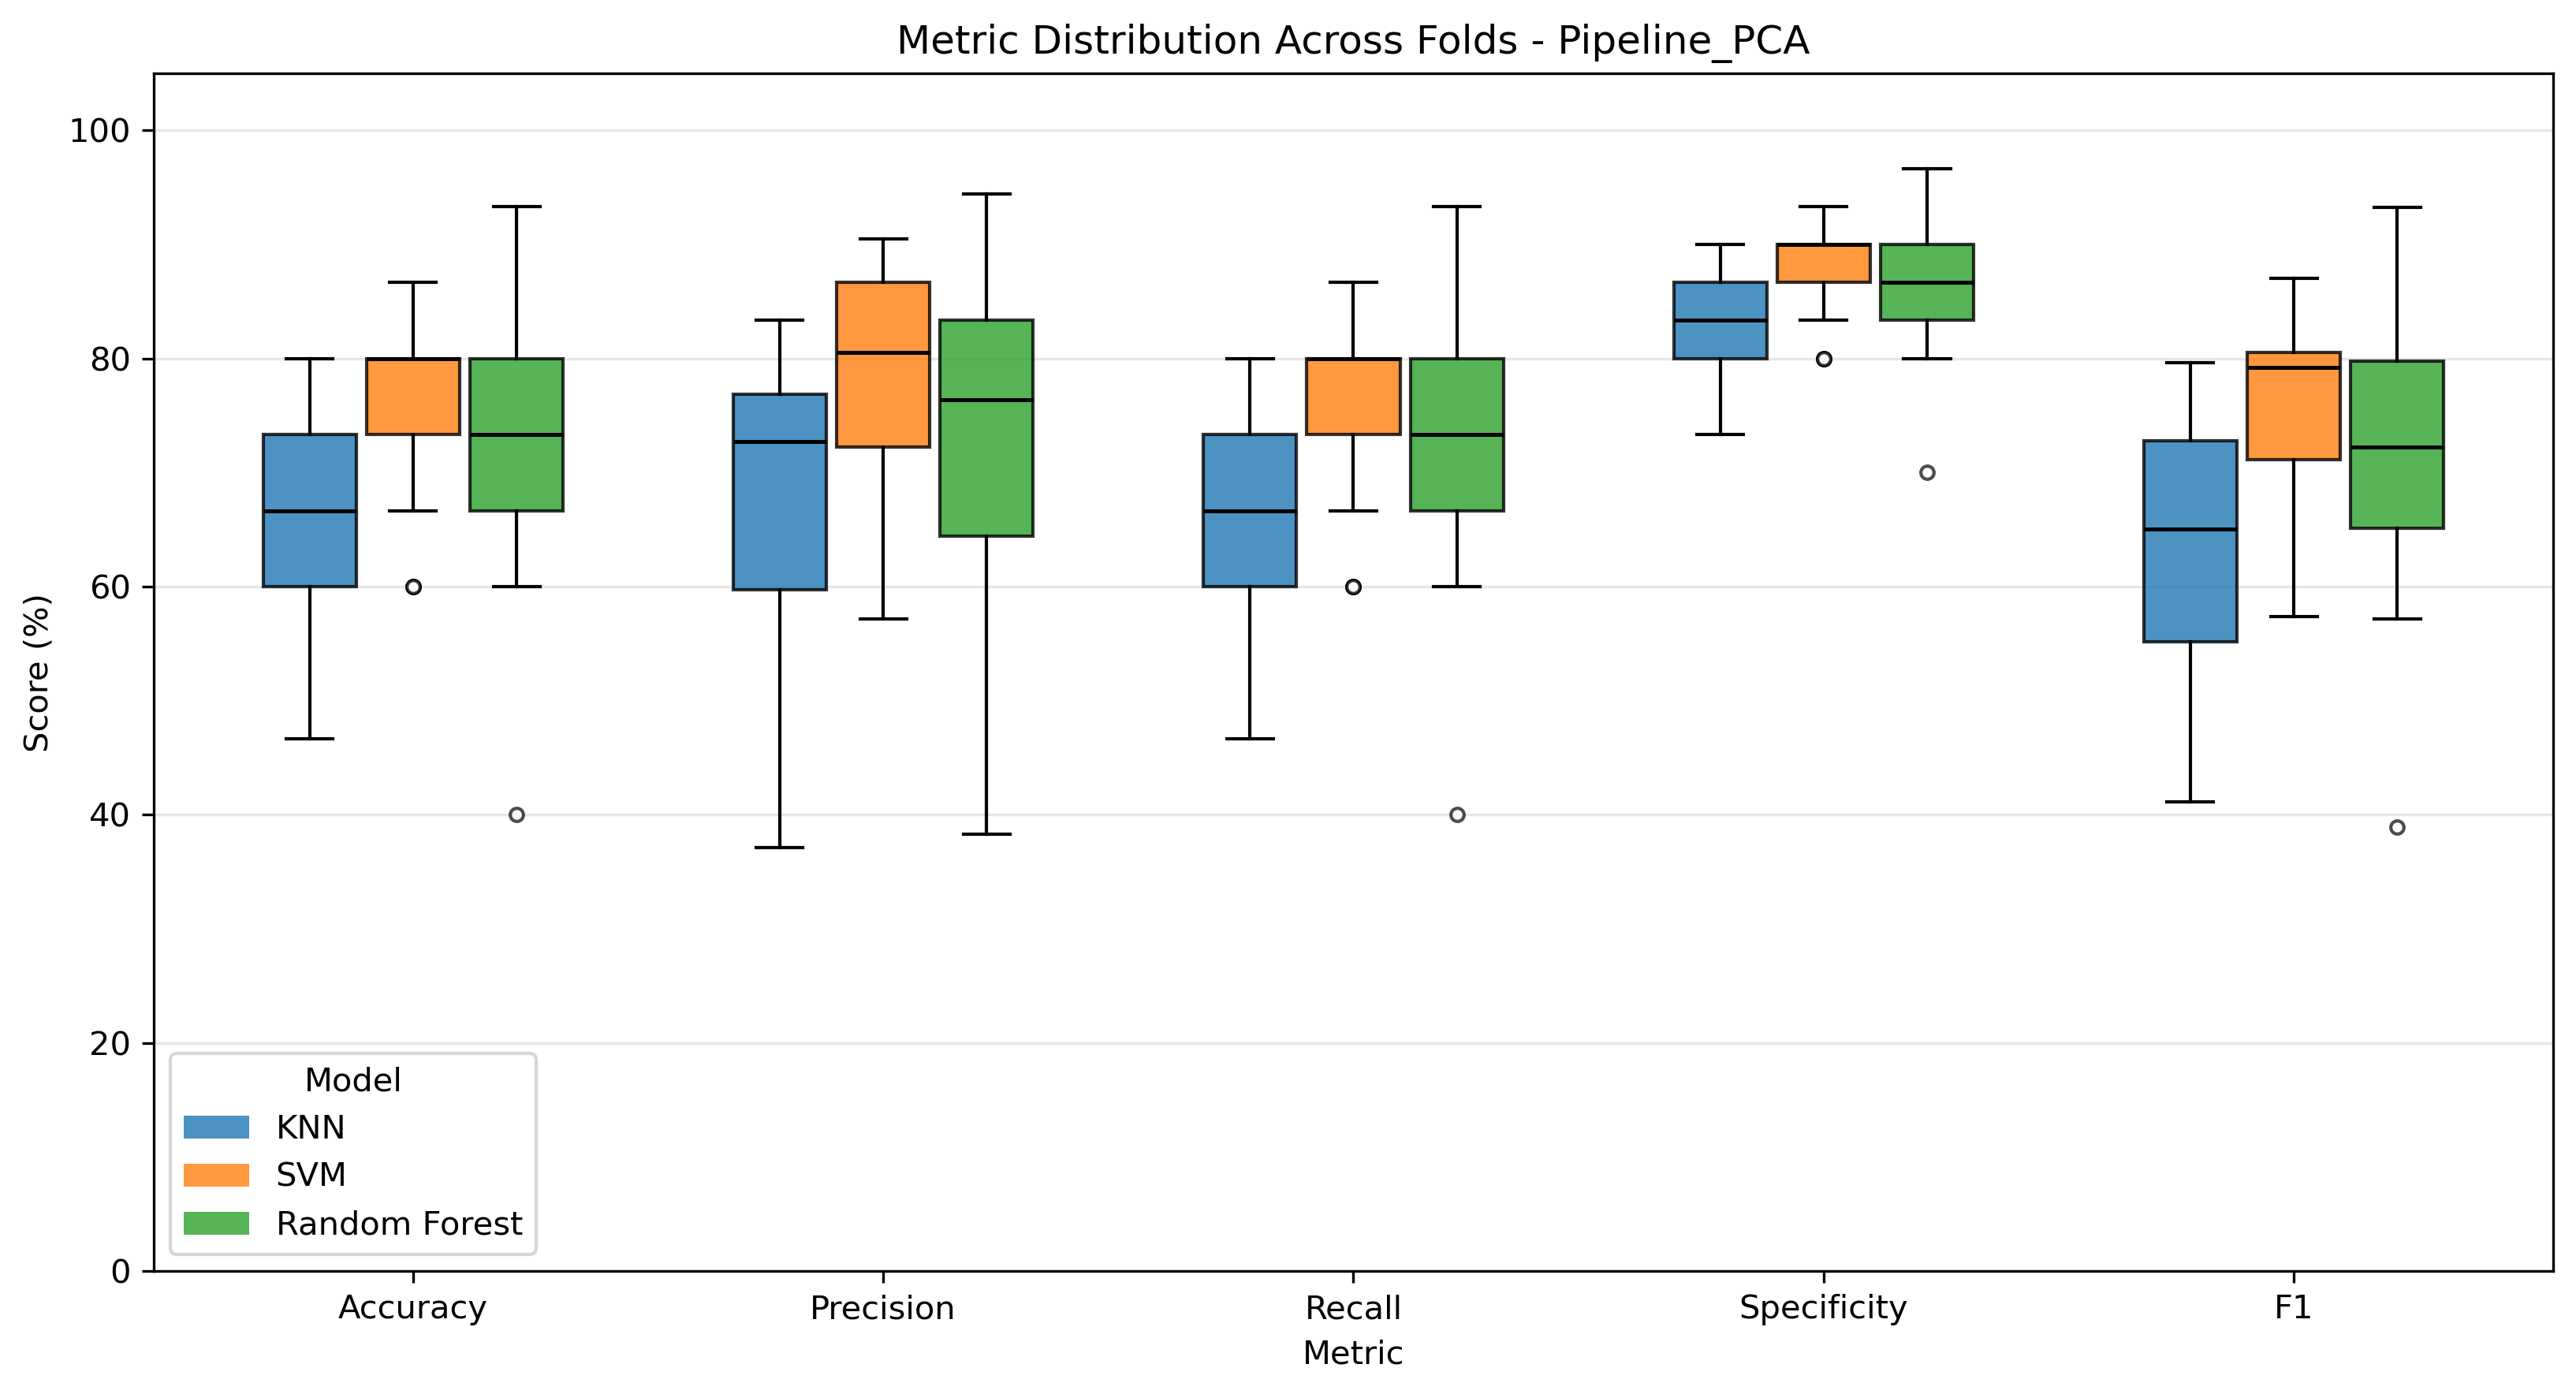
\includegraphics[width=0.7\linewidth]{../Results/Sit_To_Stand/Pipeline_PCA/Metric_Distribution_Pipeline_PCA}
	\caption{مقایسه عملکرد مدل‌های آموزش‌دیده با مؤلفه‌های اصلی در فعالیت برخاستن از زمین}
	\label{fig:Sit_To_Stand_metric_distribution_pipeline_pca}
\end{figure}

برای بررسی مستقیم اثر کاهش بعد، دقت مدل‌ها پیش و پس از اعمال تحلیل مؤلفه‌های اصلی در
\autoref{fig:Sit_To_Stand_accuracy_baseline_vs_pipeline_pca}
مقایسه شده است.

\textbf{TODO: برای هر سه مدل مشخص شود دقت افزایش یافته، کاهش یافته یا تقریباً ثابت مانده است. مدل دارای بیشترین بهبود نیز معرفی شود.}

\begin{figure}[H]
	\centering
	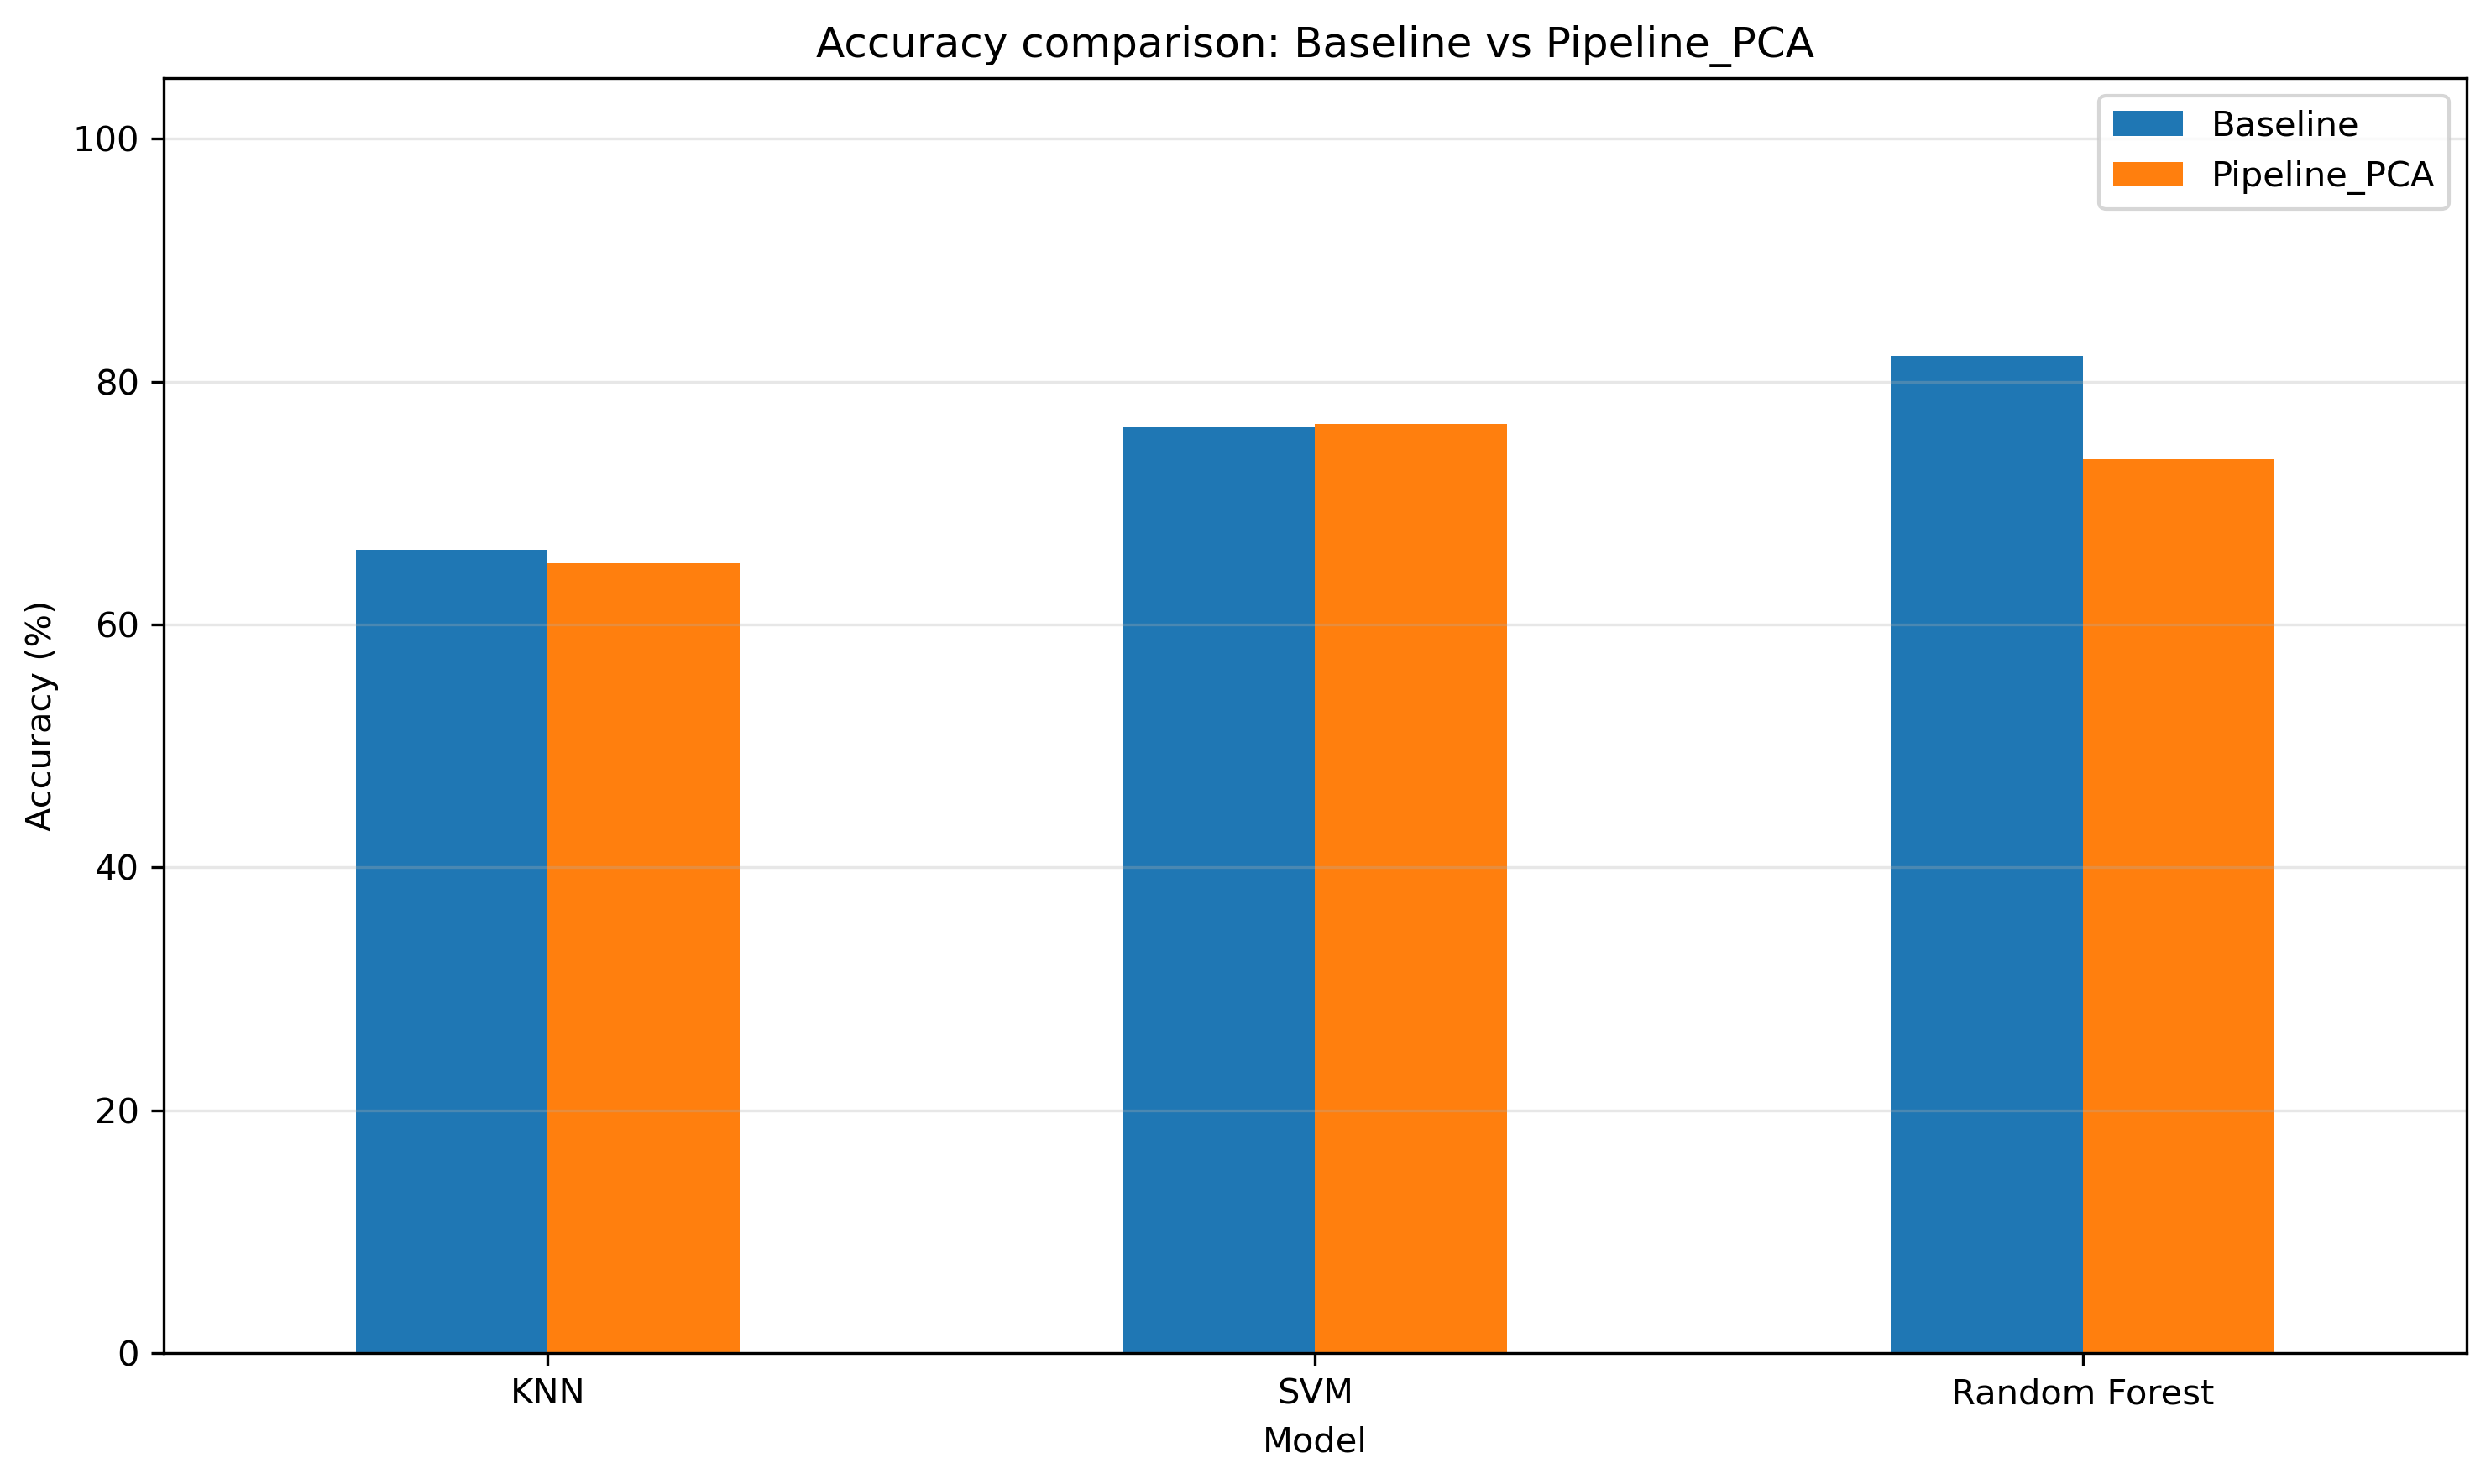
\includegraphics[width=0.7\linewidth]{../Results/Sit_To_Stand/Comparisons/Accuracy_Baseline_vs_Pipeline_PCA}
	\caption{مقایسه دقت مدل‌ها پیش و پس از کاهش بعد در فعالیت برخاستن از زمین}
	\label{fig:Sit_To_Stand_accuracy_baseline_vs_pipeline_pca}
\end{figure}

نتایج این مقایسه مشخص می‌کنند که آیا حذف اطلاعات تکراری و کاهش تعداد ورودی‌ها توانسته است تعمیم‌پذیری مدل‌ها را بهبود دهد یا خیر. همچنین مدلی که بیشترین عملکرد را پس از کاهش بعد داشته است، برای بررسی اثر تعداد مؤلفه‌های اصلی انتخاب شد.

\textbf{TODO: نام مدل انتخاب‌شده برای تحلیل تعداد مؤلفه‌ها و دلیل انتخاب آن نوشته شود.}

\subsubsection{اهمیت ویژگی‌ها و انتخاب مؤلفه‌ها}

اهمیت ویژگی‌ها بر اساس مدل جنگل تصادفی در
\autoref{fig:Sit_To_Stand_normal_rf_importance}
گزارش شده است. این نمودار نشان می‌دهد کدام ویژگی‌ها، حسگرها و محورهای حرکتی سهم بیشتری در تفکیک سه سطح عملکردی داشته‌اند.

در فعالیت برخاستن از زمین، انتظار می‌رود ویژگی‌های مرتبط با تغییر وضعیت تنه، انتقال وزن روی پاها و میزان استفاده از دست‌ها اهمیت بیشتری داشته باشند. برای مثال، ویژگی‌های دامنه، انرژی، مقادیر بیشینه و تغییرات سرعت زاویه‌ای می‌توانند اطلاعاتی درباره شدت حرکت و راهبرد مورد استفاده برای برخاستن فراهم کنند.

\textbf{TODO: نام ویژگی‌های مهم نمودار و محل حسگرهای مربوط به آن‌ها نوشته شود. همچنین مشخص شود آیا اهمیت بیشتر مربوط به دست‌ها، پاها یا سر بوده است.}

\begin{figure}[H]
	\centering
	
\includegraphics[width=0.80\linewidth]{Images/Generated/TaskResults/Sit_To_Stand/Normal/rf_top_feature_importance.png}
	\caption{ویژگی‌های مهم‌تر بر اساس مدل \lr{Random Forest} در فعالیت برخاستن از زمین}
	\label{fig:Sit_To_Stand_normal_rf_importance}
\end{figure}

اثر تعداد مؤلفه‌های اصلی بر عملکرد مدل منتخب در
\autoref{fig:Sit_To_Stand_accuracy_vs_pca_components}
ارائه شده است. این نمودار نشان می‌دهد که پس از یک تعداد مشخص از مؤلفه‌ها، افزودن مؤلفه‌های جدید لزوماً باعث افزایش قابل‌توجه دقت نمی‌شود.

\textbf{TODO: کمترین تعداد مؤلفه‌ای که با آن دقت مناسب به دست آمده و بیشترین دقت مشاهده‌شده گزارش شود.}

\begin{figure}[H]
	\centering
	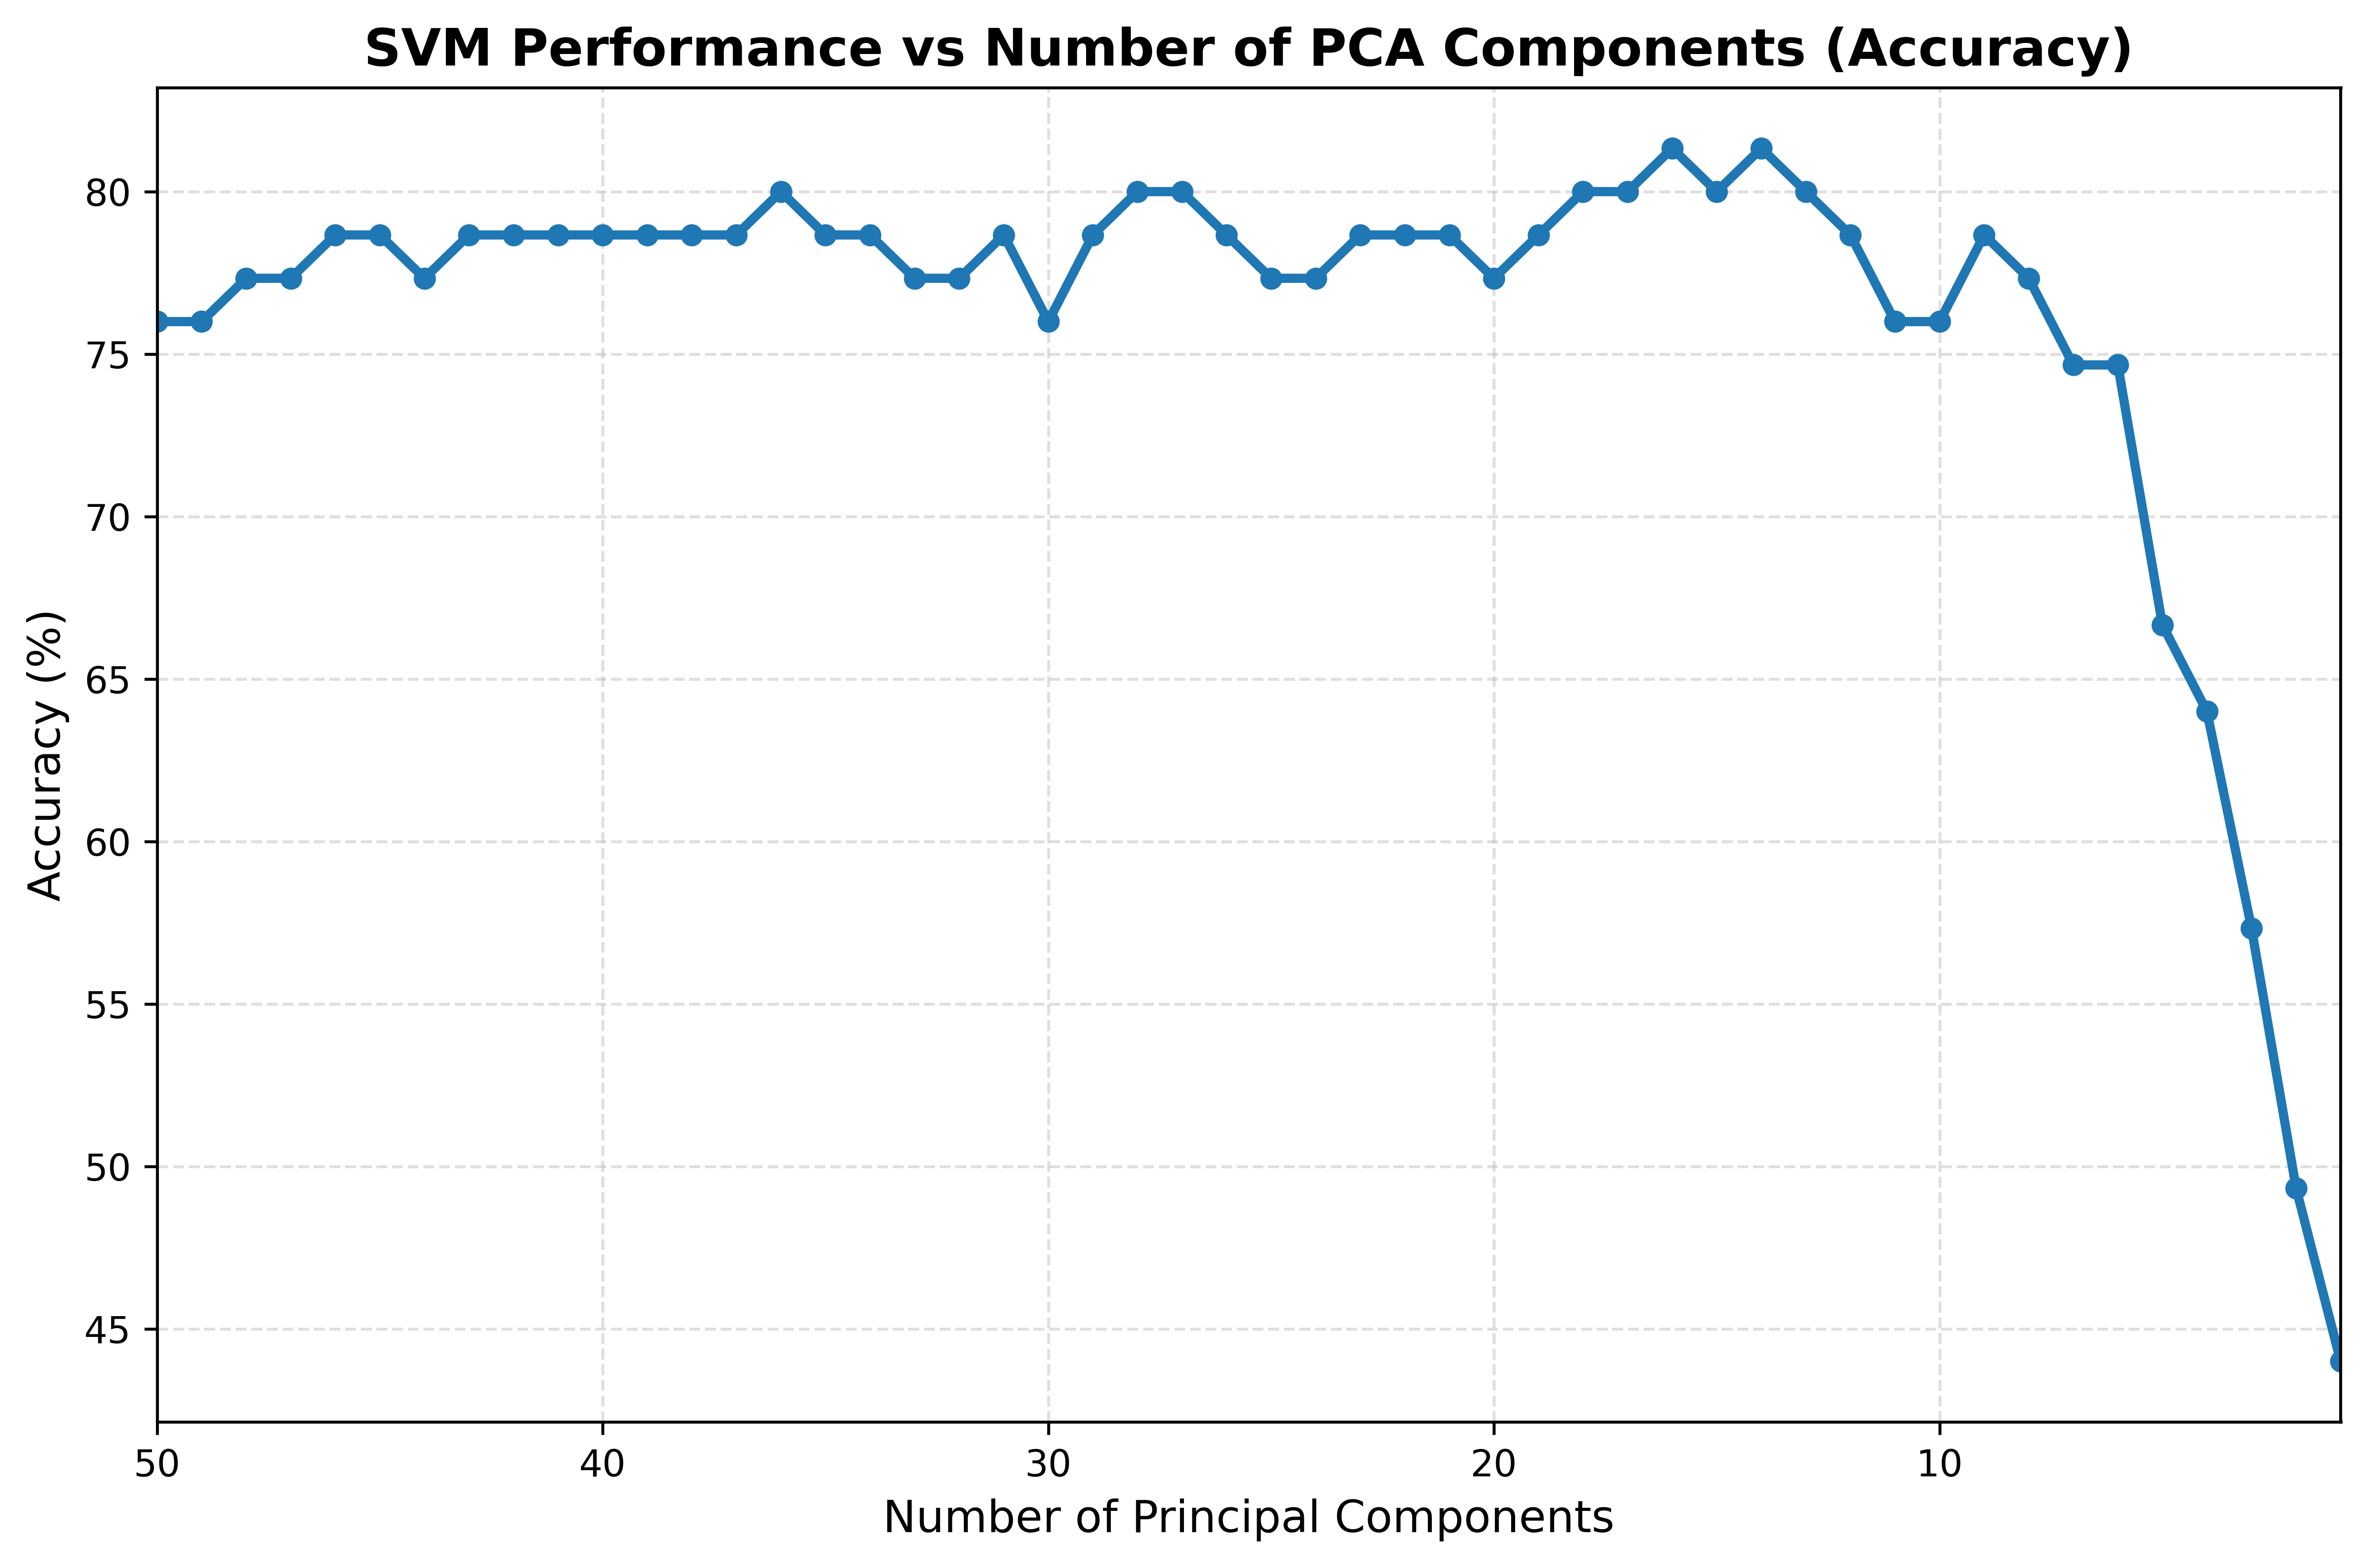
\includegraphics[width=0.8\linewidth]{../Results/Sit_To_Stand/Normal/FindPrincipalComponents_PipelinePCA_Sit_To_Stand/Figures/Accuracy_vs_PCA}
	\caption{تغییر دقت مدل منتخب نسبت به تعداد مؤلفه‌های اصلی در فعالیت برخاستن از زمین}
	\label{fig:Sit_To_Stand_accuracy_vs_pca_components}
\end{figure}

در
\autoref{fig:Sit_To_Stand_all_metrics_vs_pca}
تغییرات تمام معیارهای ارزیابی نسبت به تعداد مؤلفه‌های اصلی نمایش داده شده است. بررسی هم‌زمان این معیارها از انتخاب حالتی جلوگیری می‌کند که تنها دارای دقت بالا باشد، اما در شناسایی یکی از طبقه‌ها عملکرد ضعیفی داشته باشد.

\textbf{TODO: مشخص شود آیا معیارهای مختلف روند مشابهی داشته‌اند یا خیر. تعداد مؤلفه مربوط به بهترین امتیاز F1، بازخوانی و دقت نیز در صورت متفاوت‌بودن گزارش شود.}

\begin{figure}[H]
	\centering
	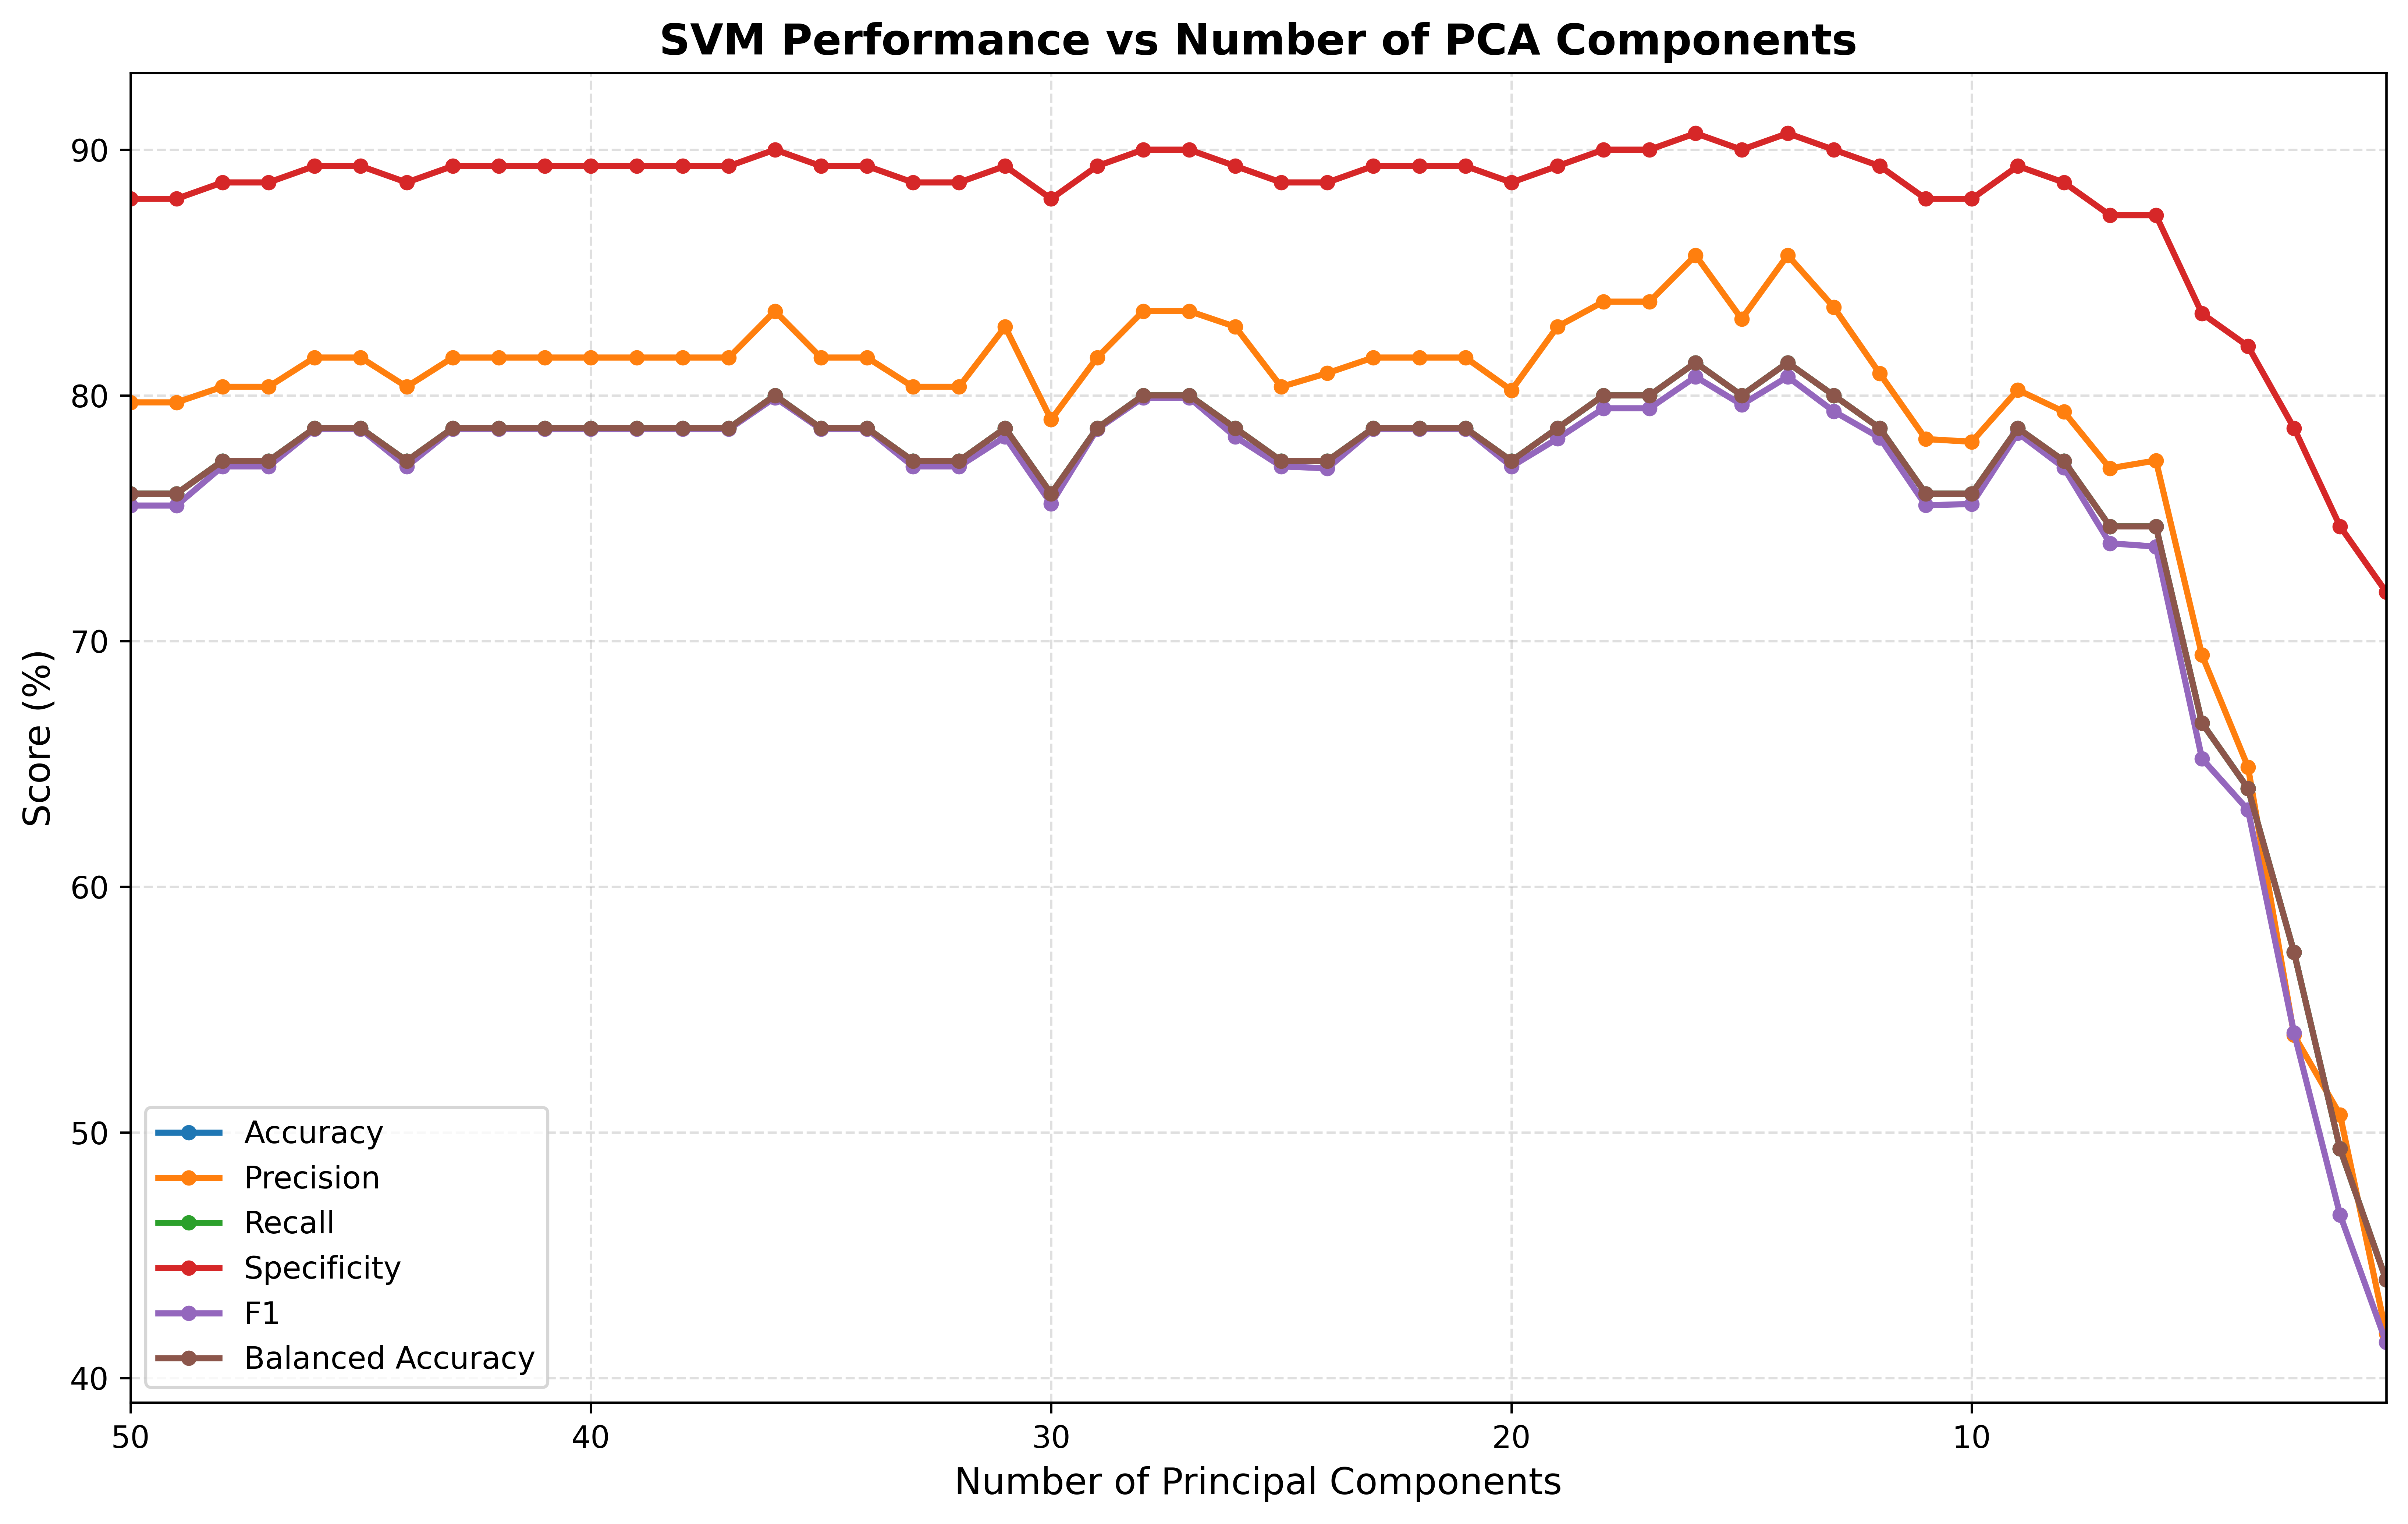
\includegraphics[width=0.8\linewidth]{../Results/Sit_To_Stand/Normal/FindPrincipalComponents_PipelinePCA_Sit_To_Stand/Figures/All_Metrics_vs_PCA}
	\caption{تغییر عملکرد مدل منتخب نسبت به تعداد مؤلفه‌های اصلی در فعالیت برخاستن از زمین}
	\label{fig:Sit_To_Stand_all_metrics_vs_pca}
\end{figure}

در نهایت، بر اساس نمودارهای
\autoref{fig:Sit_To_Stand_accuracy_vs_pca_components}
و
\autoref{fig:Sit_To_Stand_all_metrics_vs_pca}،
مدل‌ها در بازه
\textbf{TODO: بازه تعداد مؤلفه‌ها}
دوباره مقایسه شدند تا مدل برتر و تعداد مؤلفه‌های اصلی بهینه تعیین شود. نتیجه این مقایسه در
\autoref{fig:Sit_To_Stand_models_vs_pca_components}
ارائه شده است.

بر اساس این نتایج، برای فعالیت برخاستن از زمین مدل
\textbf{TODO: نام مدل منتخب}
با
\textbf{TODO: تعداد مؤلفه اصلی}
مؤلفه اصلی انتخاب شد.

\begin{figure}[H]
	\centering
	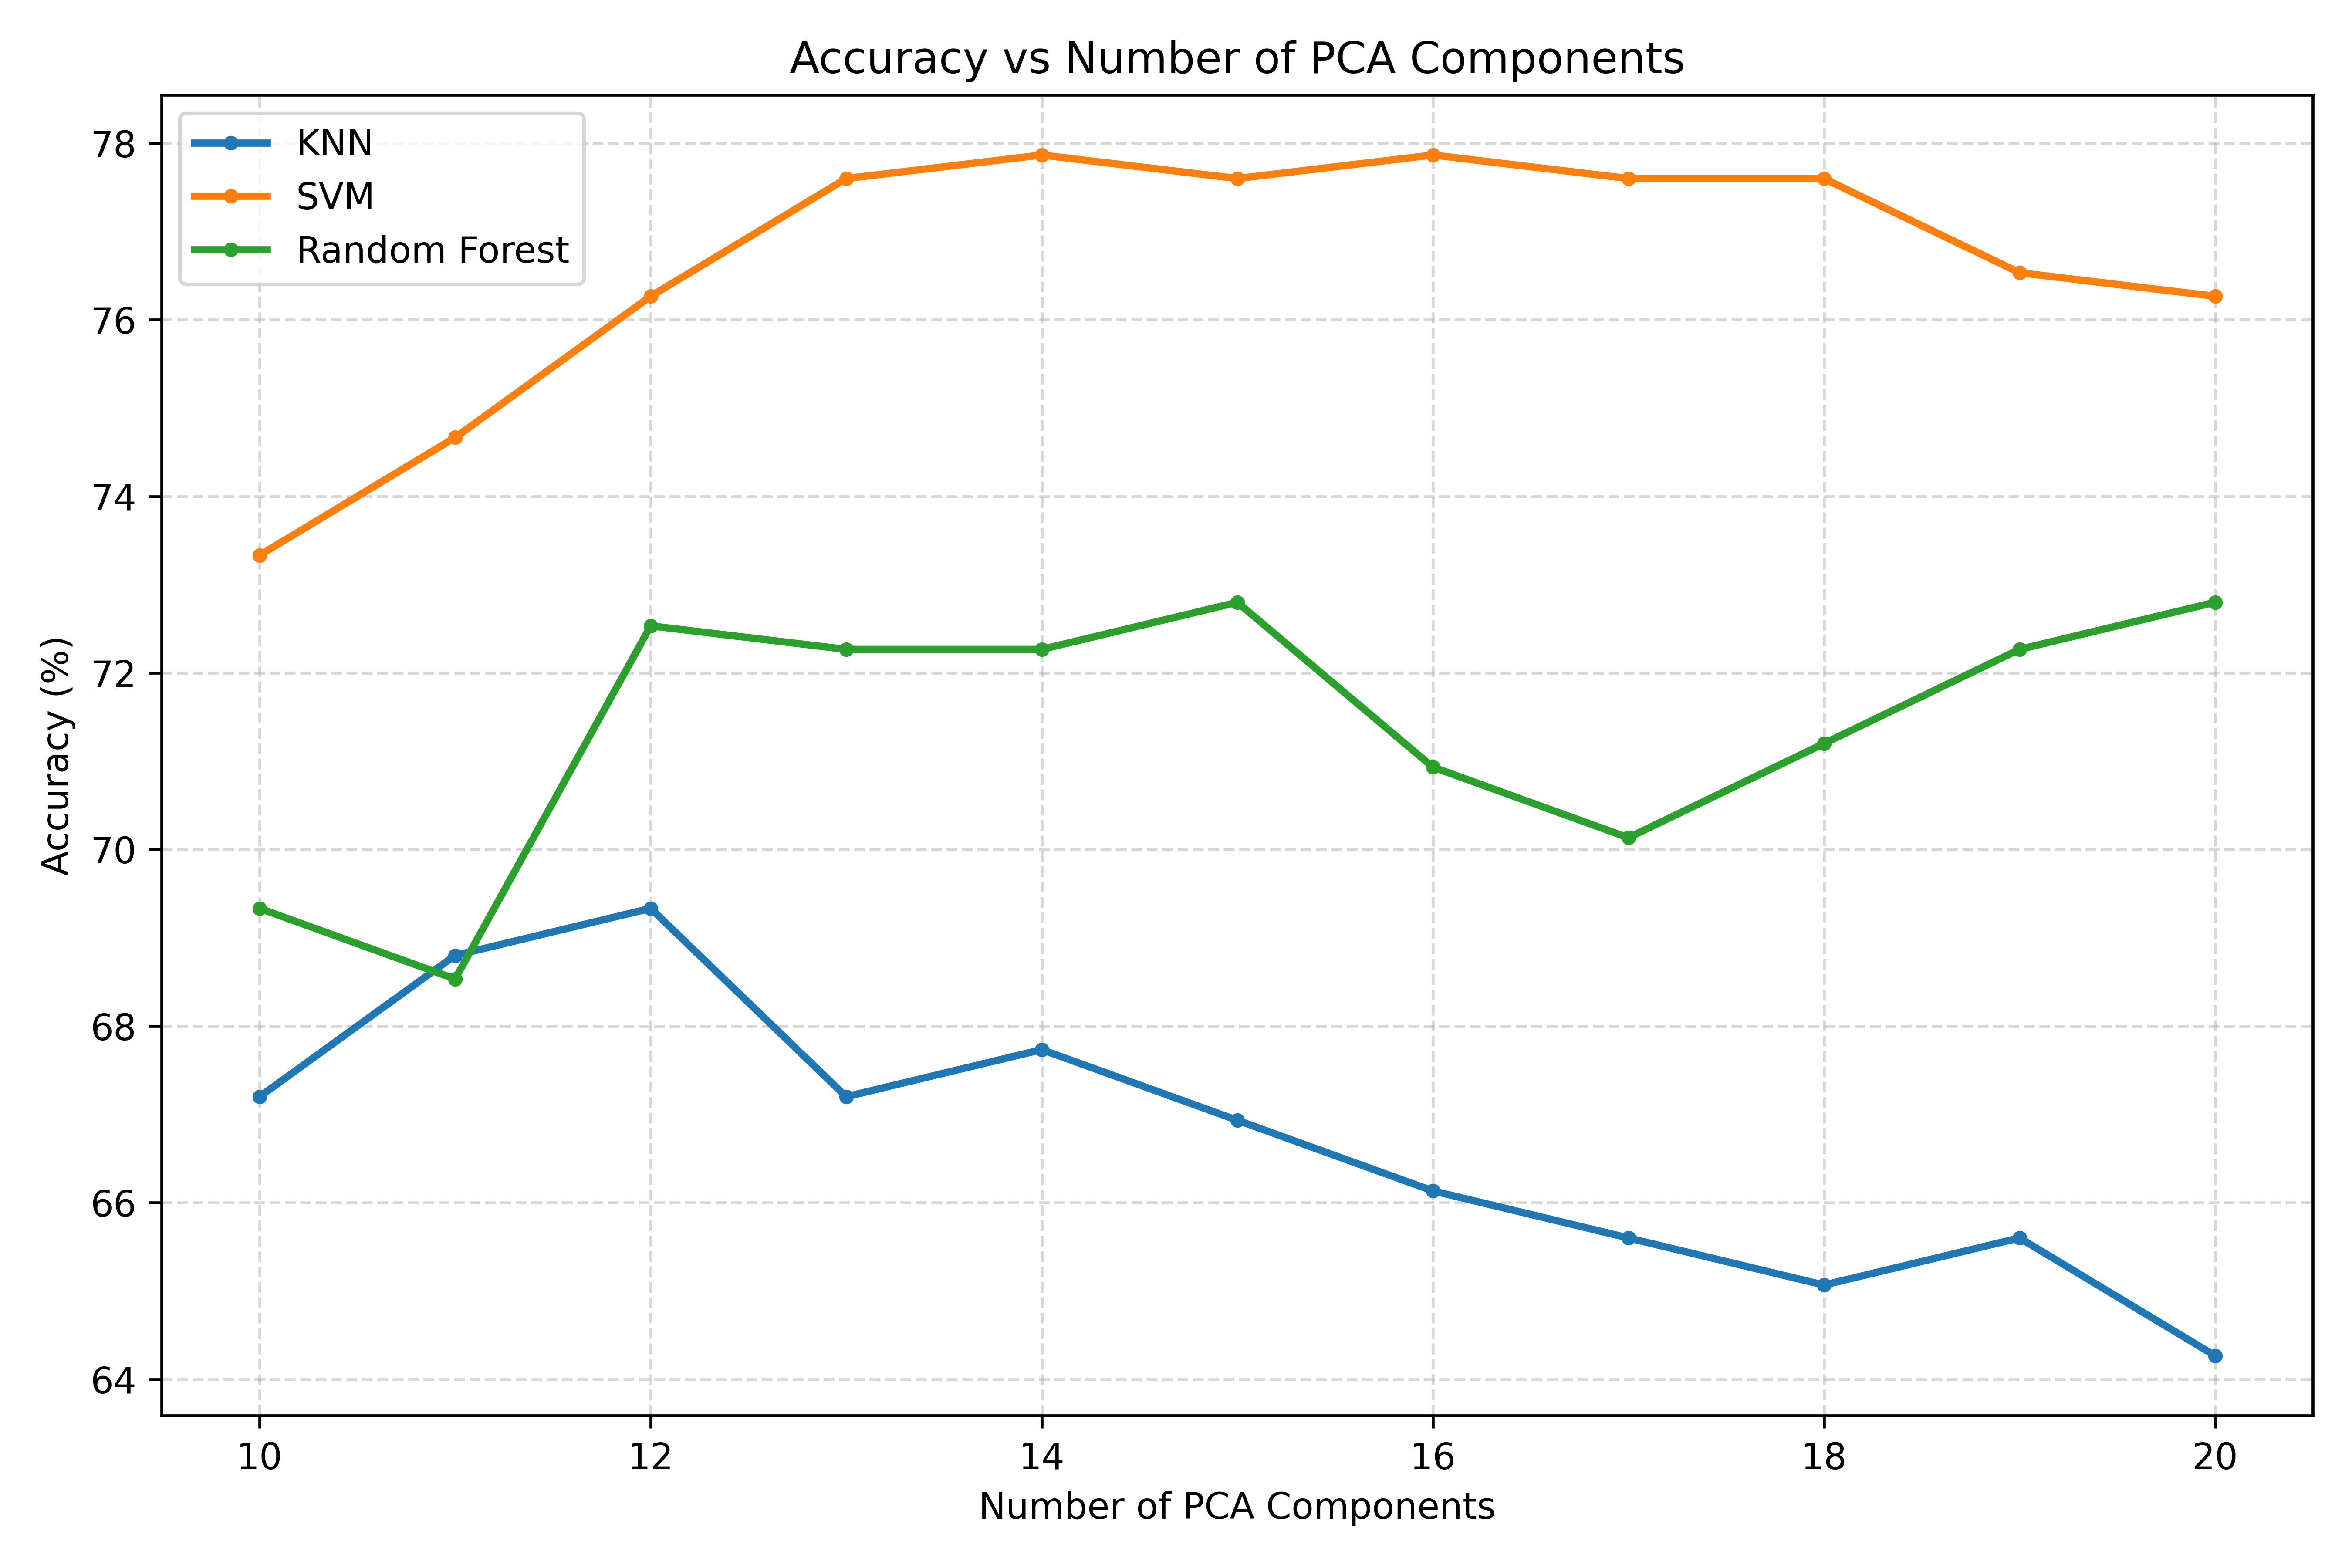
\includegraphics[width=0.8\linewidth]{../Results/Sit_To_Stand/Normal/CompareNumberOfPrincipalComponents_PipelinePCA_Sit_To_Stand/Figures/Accuracy_vs_PCA_Components}
	\caption{تغییر دقت مدل‌ها نسبت به تعداد مؤلفه‌های اصلی در فعالیت برخاستن از زمین}
	\label{fig:Sit_To_Stand_models_vs_pca_components}
\end{figure}

\begin{table}[H]
	\centering
	\caption{تنظیمات منتخب فعالیت برخاستن از زمین برای مدل نهایی}
	\label{tab:Sit_To_Stand_selected_setup}
	\begin{tabular}{lcc}
		\toprule
		مدل منتخب & نوع داده & تعداد مؤلفه اصلی \\
		\midrule
		\textbf{TODO: مدل منتخب} &
		\textbf{TODO: داده کامل یا جداسازی‌شده} &
		\textbf{TODO: تعداد مؤلفه} \\
		\bottomrule
	\end{tabular}
\end{table}

نتیجه نهایی با توجه به تنظیمات ذکرشده در
\autoref{tab:Sit_To_Stand_selected_setup}
در
\autoref{fig:Sit_To_Stand_final_model_metrics}
ارائه شده است.

\begin{figure}[H]
	\centering
	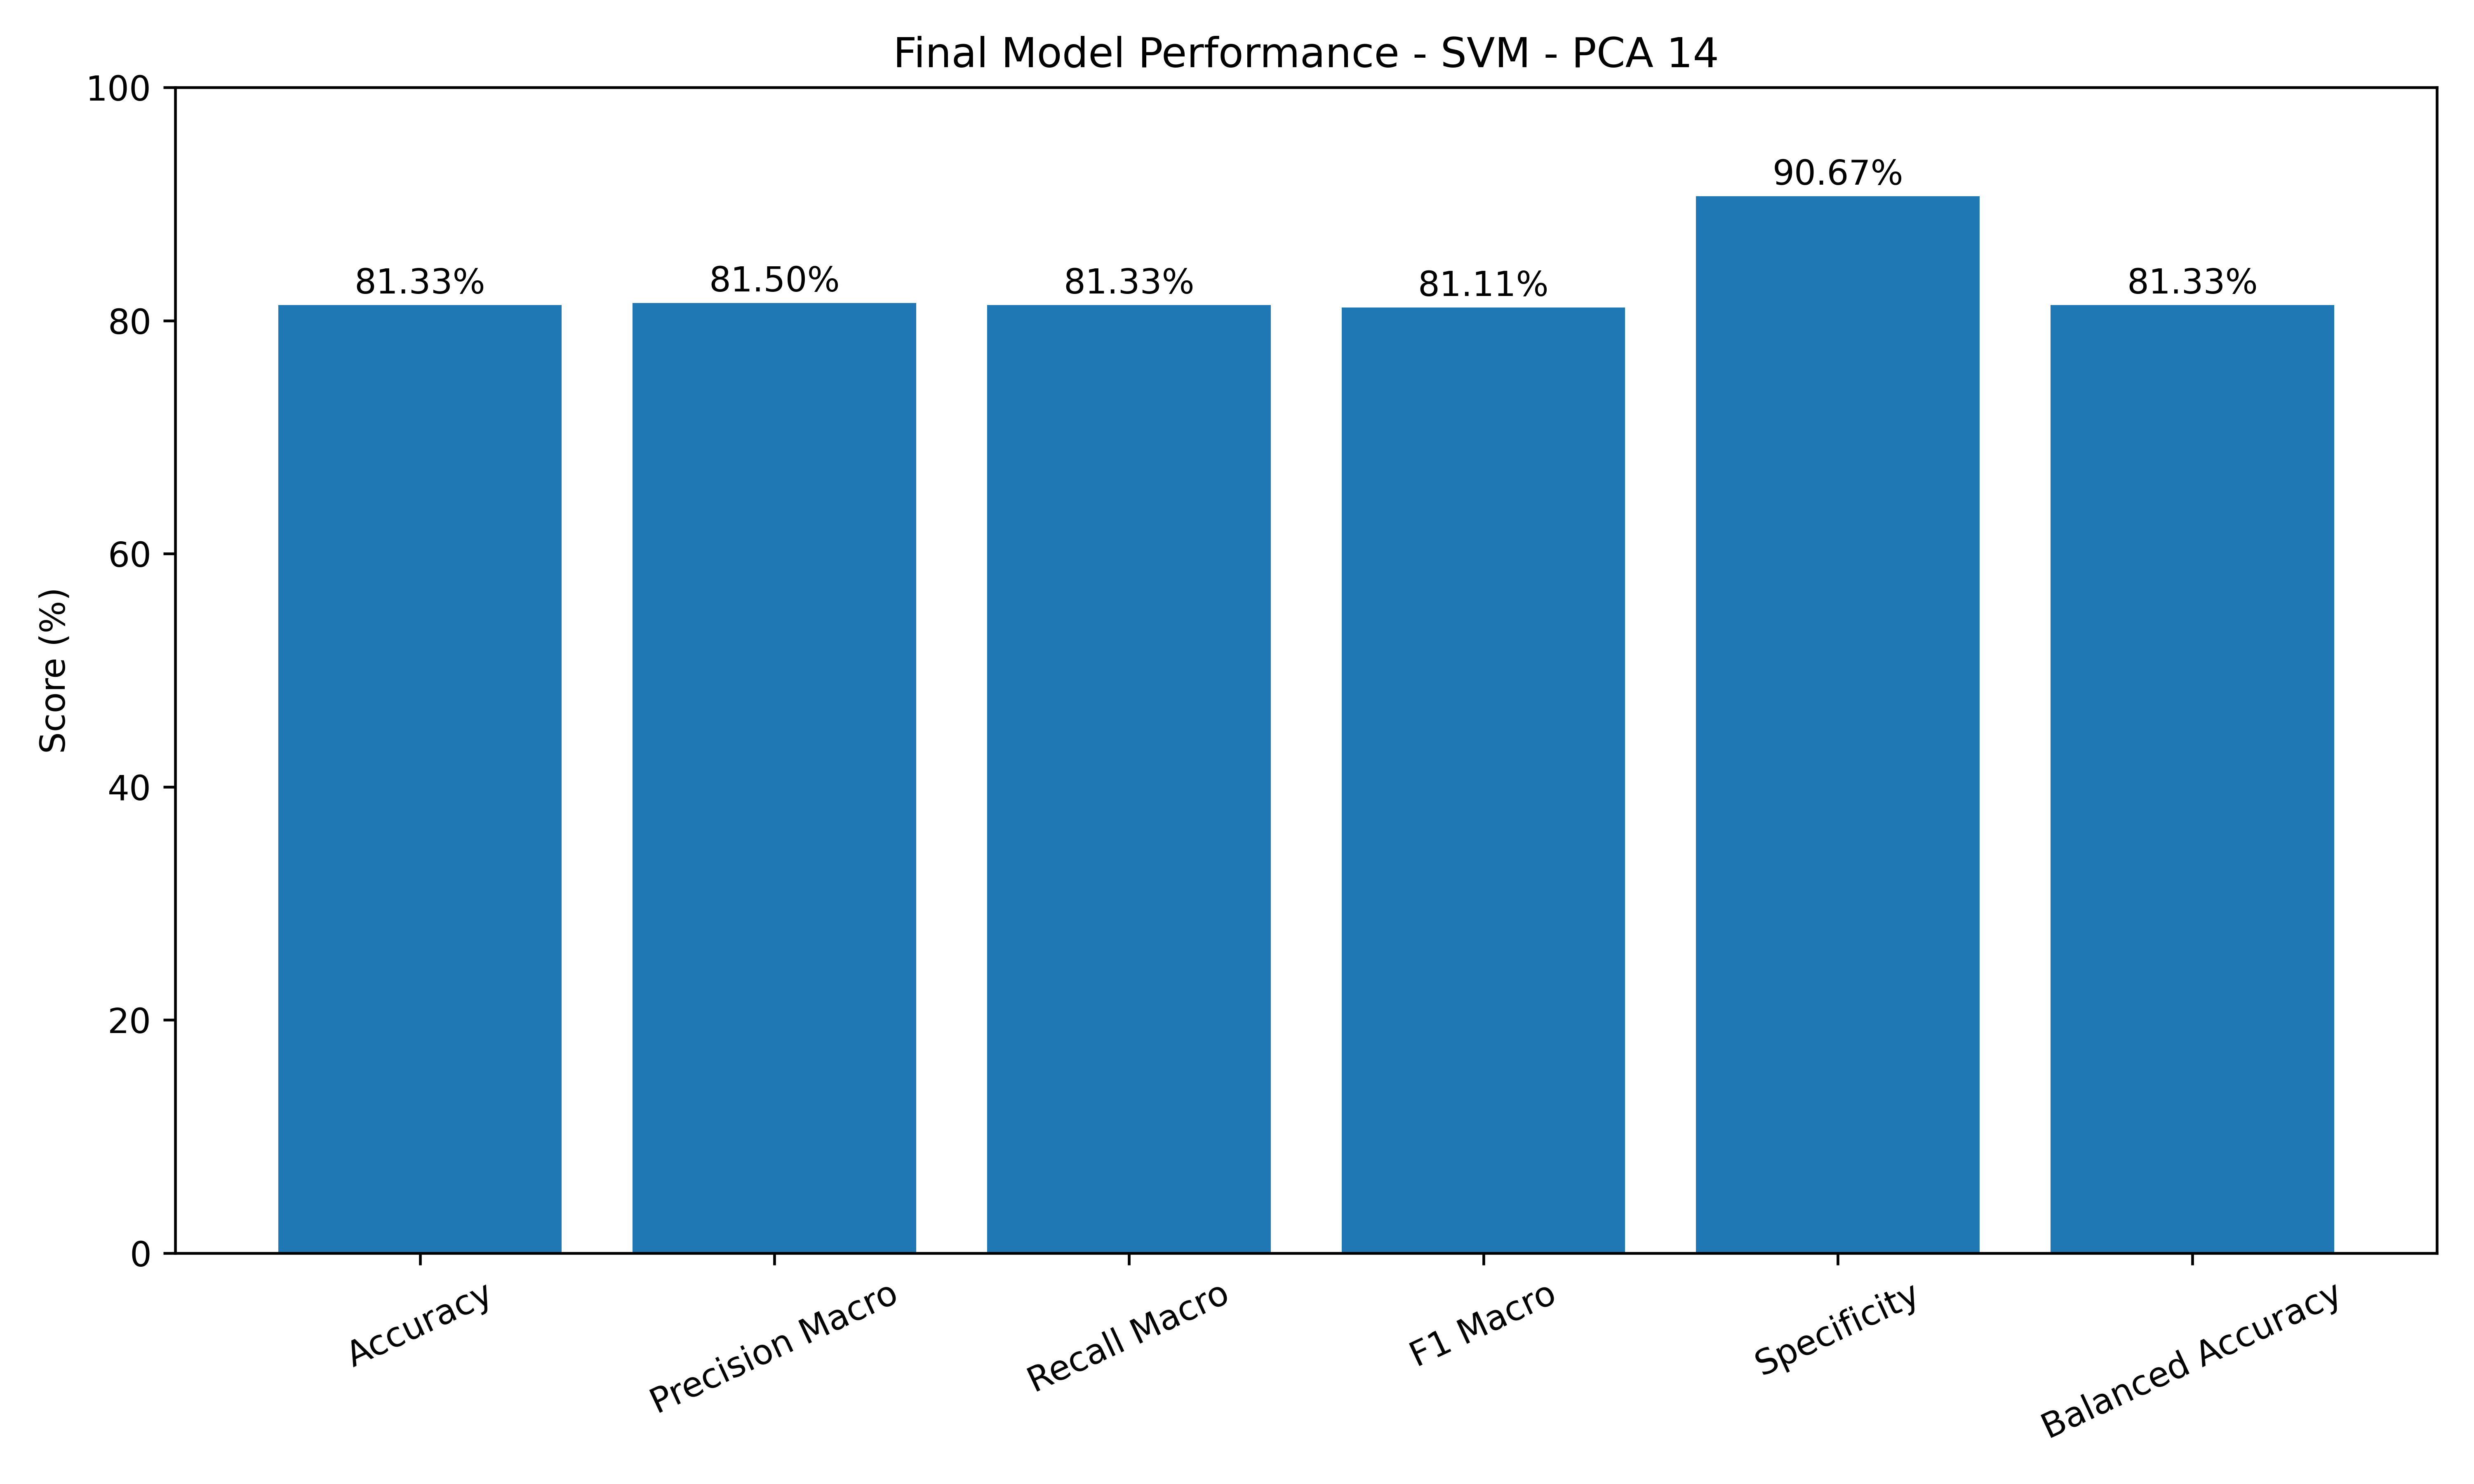
\includegraphics[width=0.8\linewidth]{../Results/Sit_To_Stand/Final/Final_Model_SVM_PCA14/Figures/Final_Model_Main_Metrics_Bar}
	\caption{عملکرد مدل نهایی منتخب در فعالیت برخاستن از زمین}
	\label{fig:Sit_To_Stand_final_model_metrics}
\end{figure}

\subsubsection{جمع‌بندی فعالیت برخاستن از زمین}

در فعالیت برخاستن از زمین، مدل منتخب معرفی‌شده در
\autoref{tab:Sit_To_Stand_selected_setup}
با استفاده از اعتبارسنجی متقاطع طبقه‌بندی‌شده مورد ارزیابی قرار گرفت. نتایج نشان می‌دهند که ویژگی‌های حرکتی استخراج‌شده از حسگرها قابلیت استفاده برای تفکیک سه سطح عملکردی شبیه‌سازی‌شده این فعالیت را دارند.

توزیع واریانس مؤلفه‌های اصلی منتخب در
\autoref{fig:Sit_To_Stand_pca_explained_variance}
ارائه شده است. مؤلفه‌های انتخاب‌شده در مجموع حدود
\textbf{TODO: درصد واریانس حفظ‌شده}
از واریانس داده‌های اولیه را در بر می‌گیرند. این نتیجه نشان می‌دهد که برای دستیابی به عملکرد مناسب مدل، حفظ تمام واریانس داده‌ها ضروری نبوده است.

\begin{figure}[H]
	\centering
	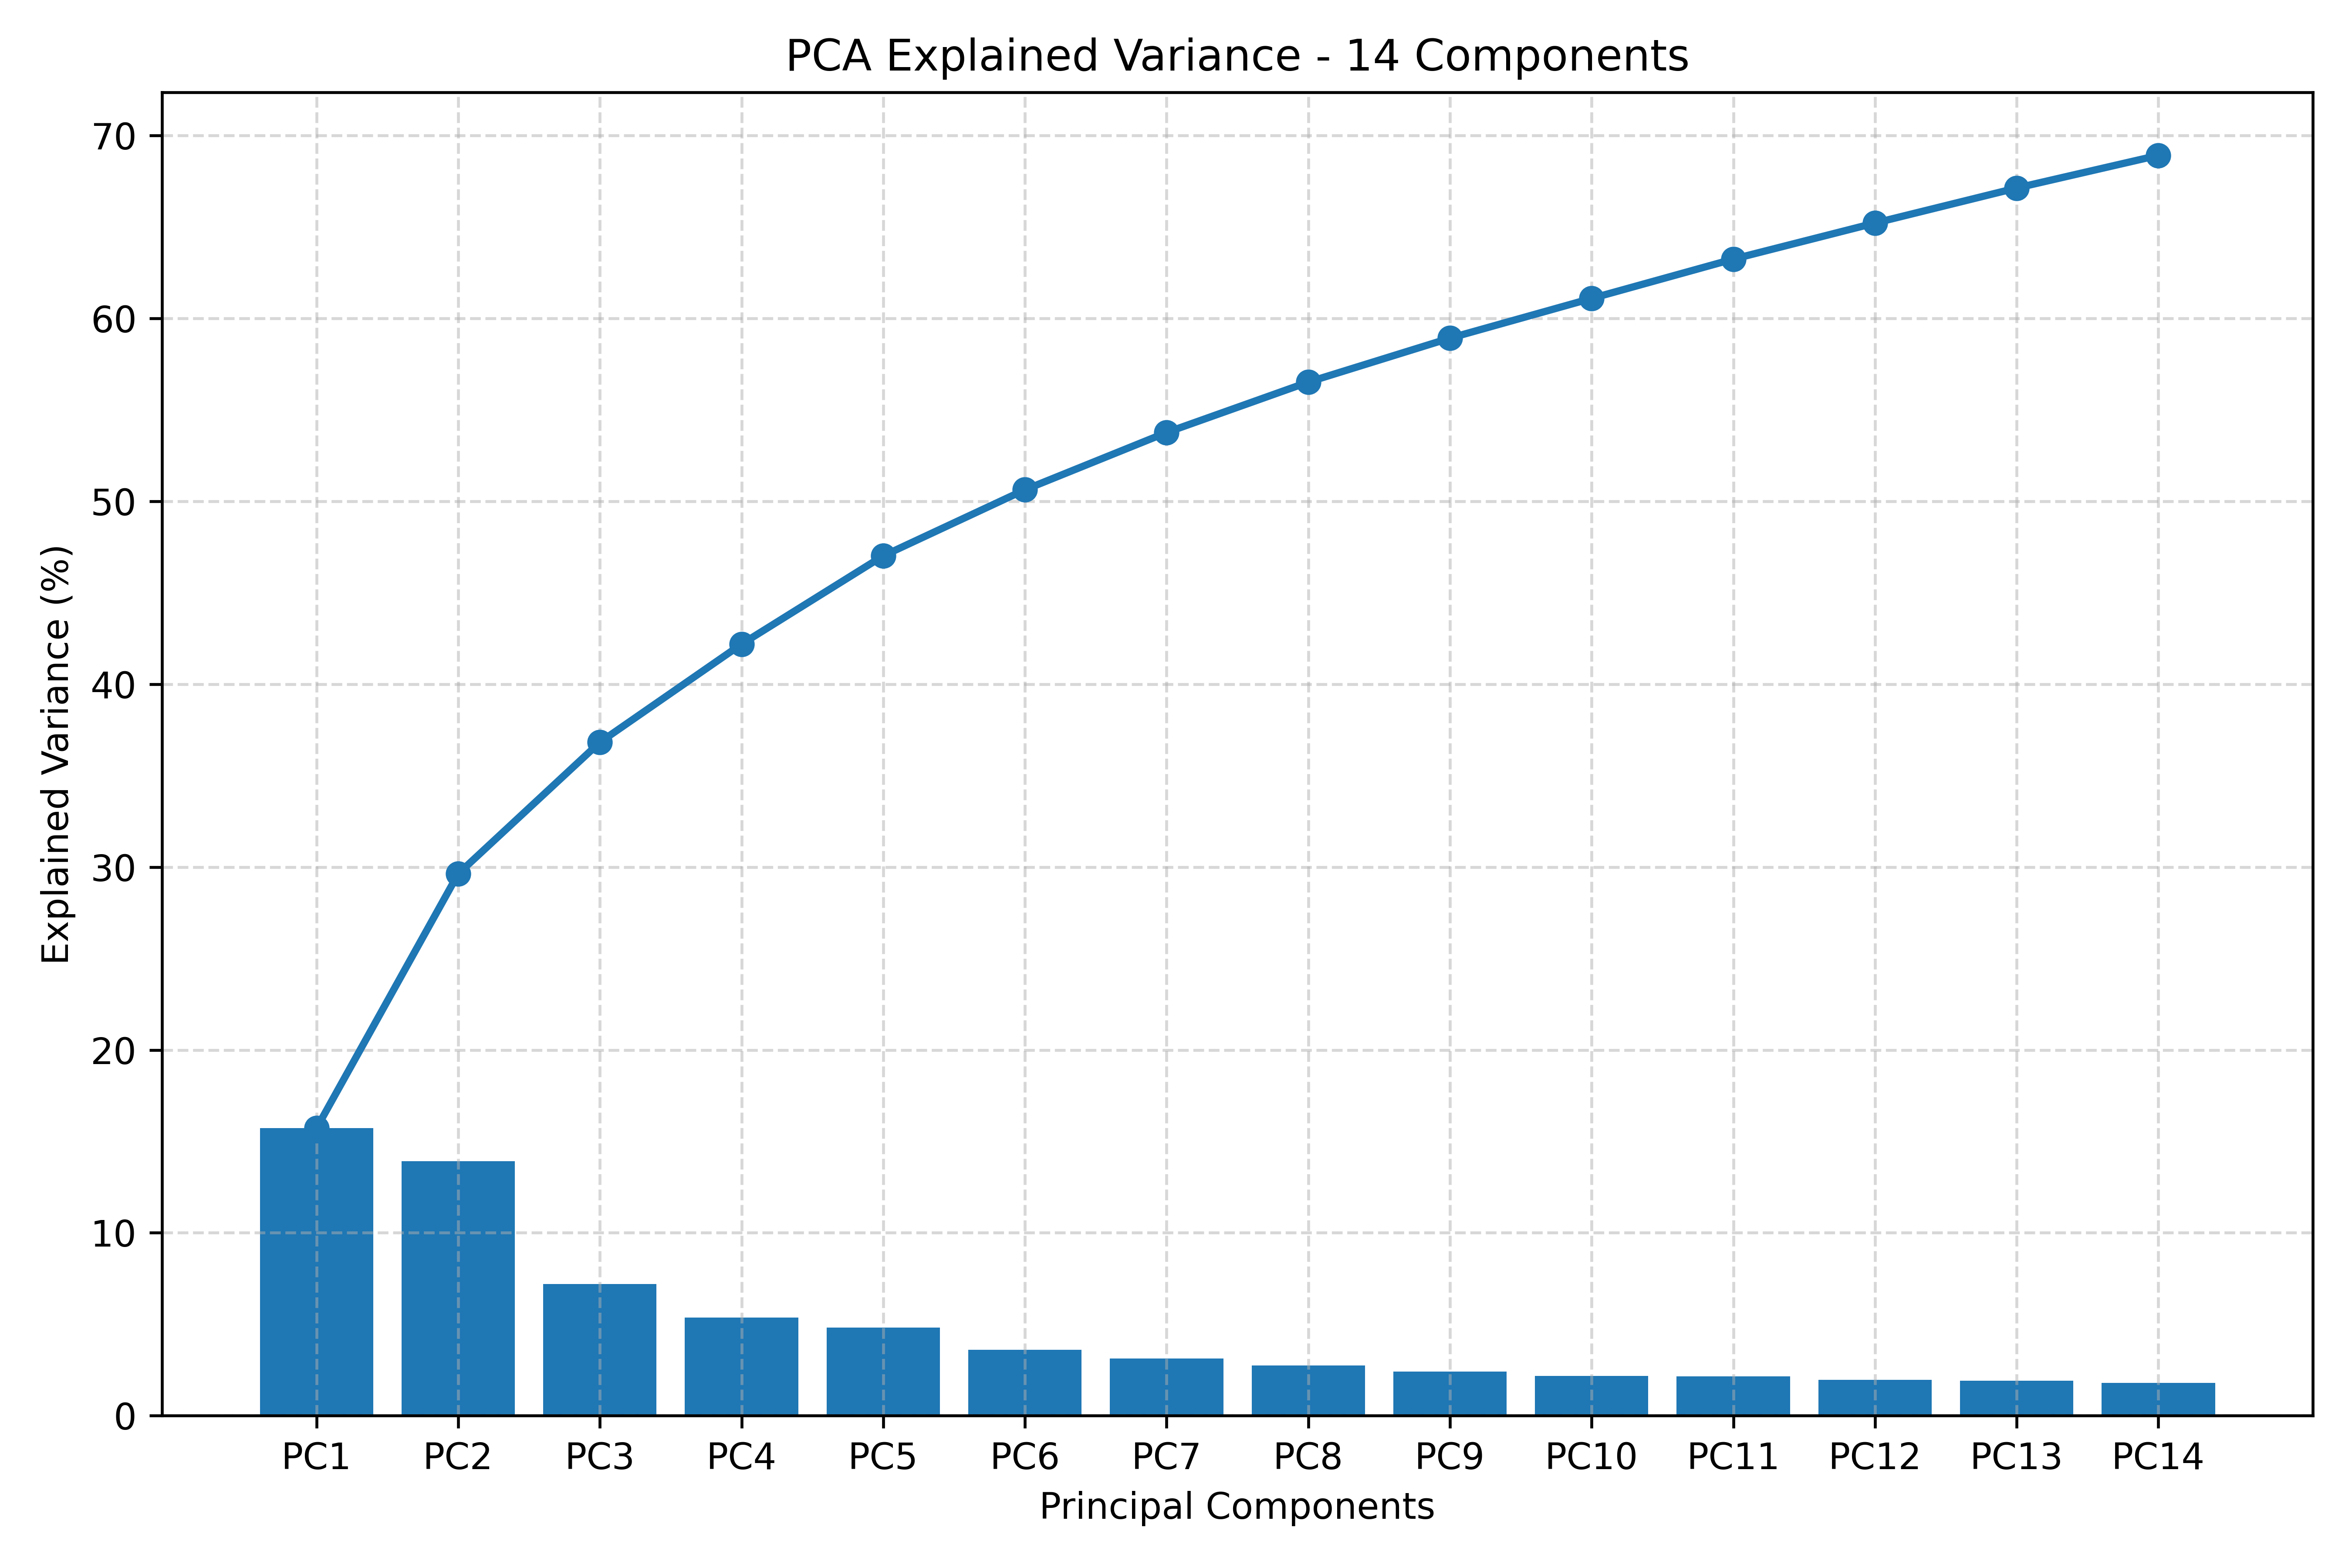
\includegraphics[width=0.8\linewidth]{../Results/Sit_To_Stand/Final/Final_Model_SVM_PCA14/Figures/PCA_Explained_Variance}
	\caption{توزیع واریانس مؤلفه‌های اصلی منتخب برای فعالیت برخاستن از زمین}
	\label{fig:Sit_To_Stand_pca_explained_variance}
\end{figure}

در این ارزیابی، داده‌ها در هر مرحله به
\textbf{TODO: تعداد بخش‌های اعتبارسنجی}
بخش تقسیم شدند و فرایند اعتبارسنجی
\textbf{TODO: تعداد تکرار}
مرتبه تکرار شد. نتایج حاصل از تقسیم‌بندی‌های مختلف در
\autoref{fig:Sit_To_Stand_cv_fold_metrics}
آمده‌اند.

\textbf{TODO: میزان ثبات نتایج در تکرارهای مختلف و معیار دارای بیشترین یا کمترین پراکندگی توضیح داده شود.}

\begin{figure}[H]
	\centering
	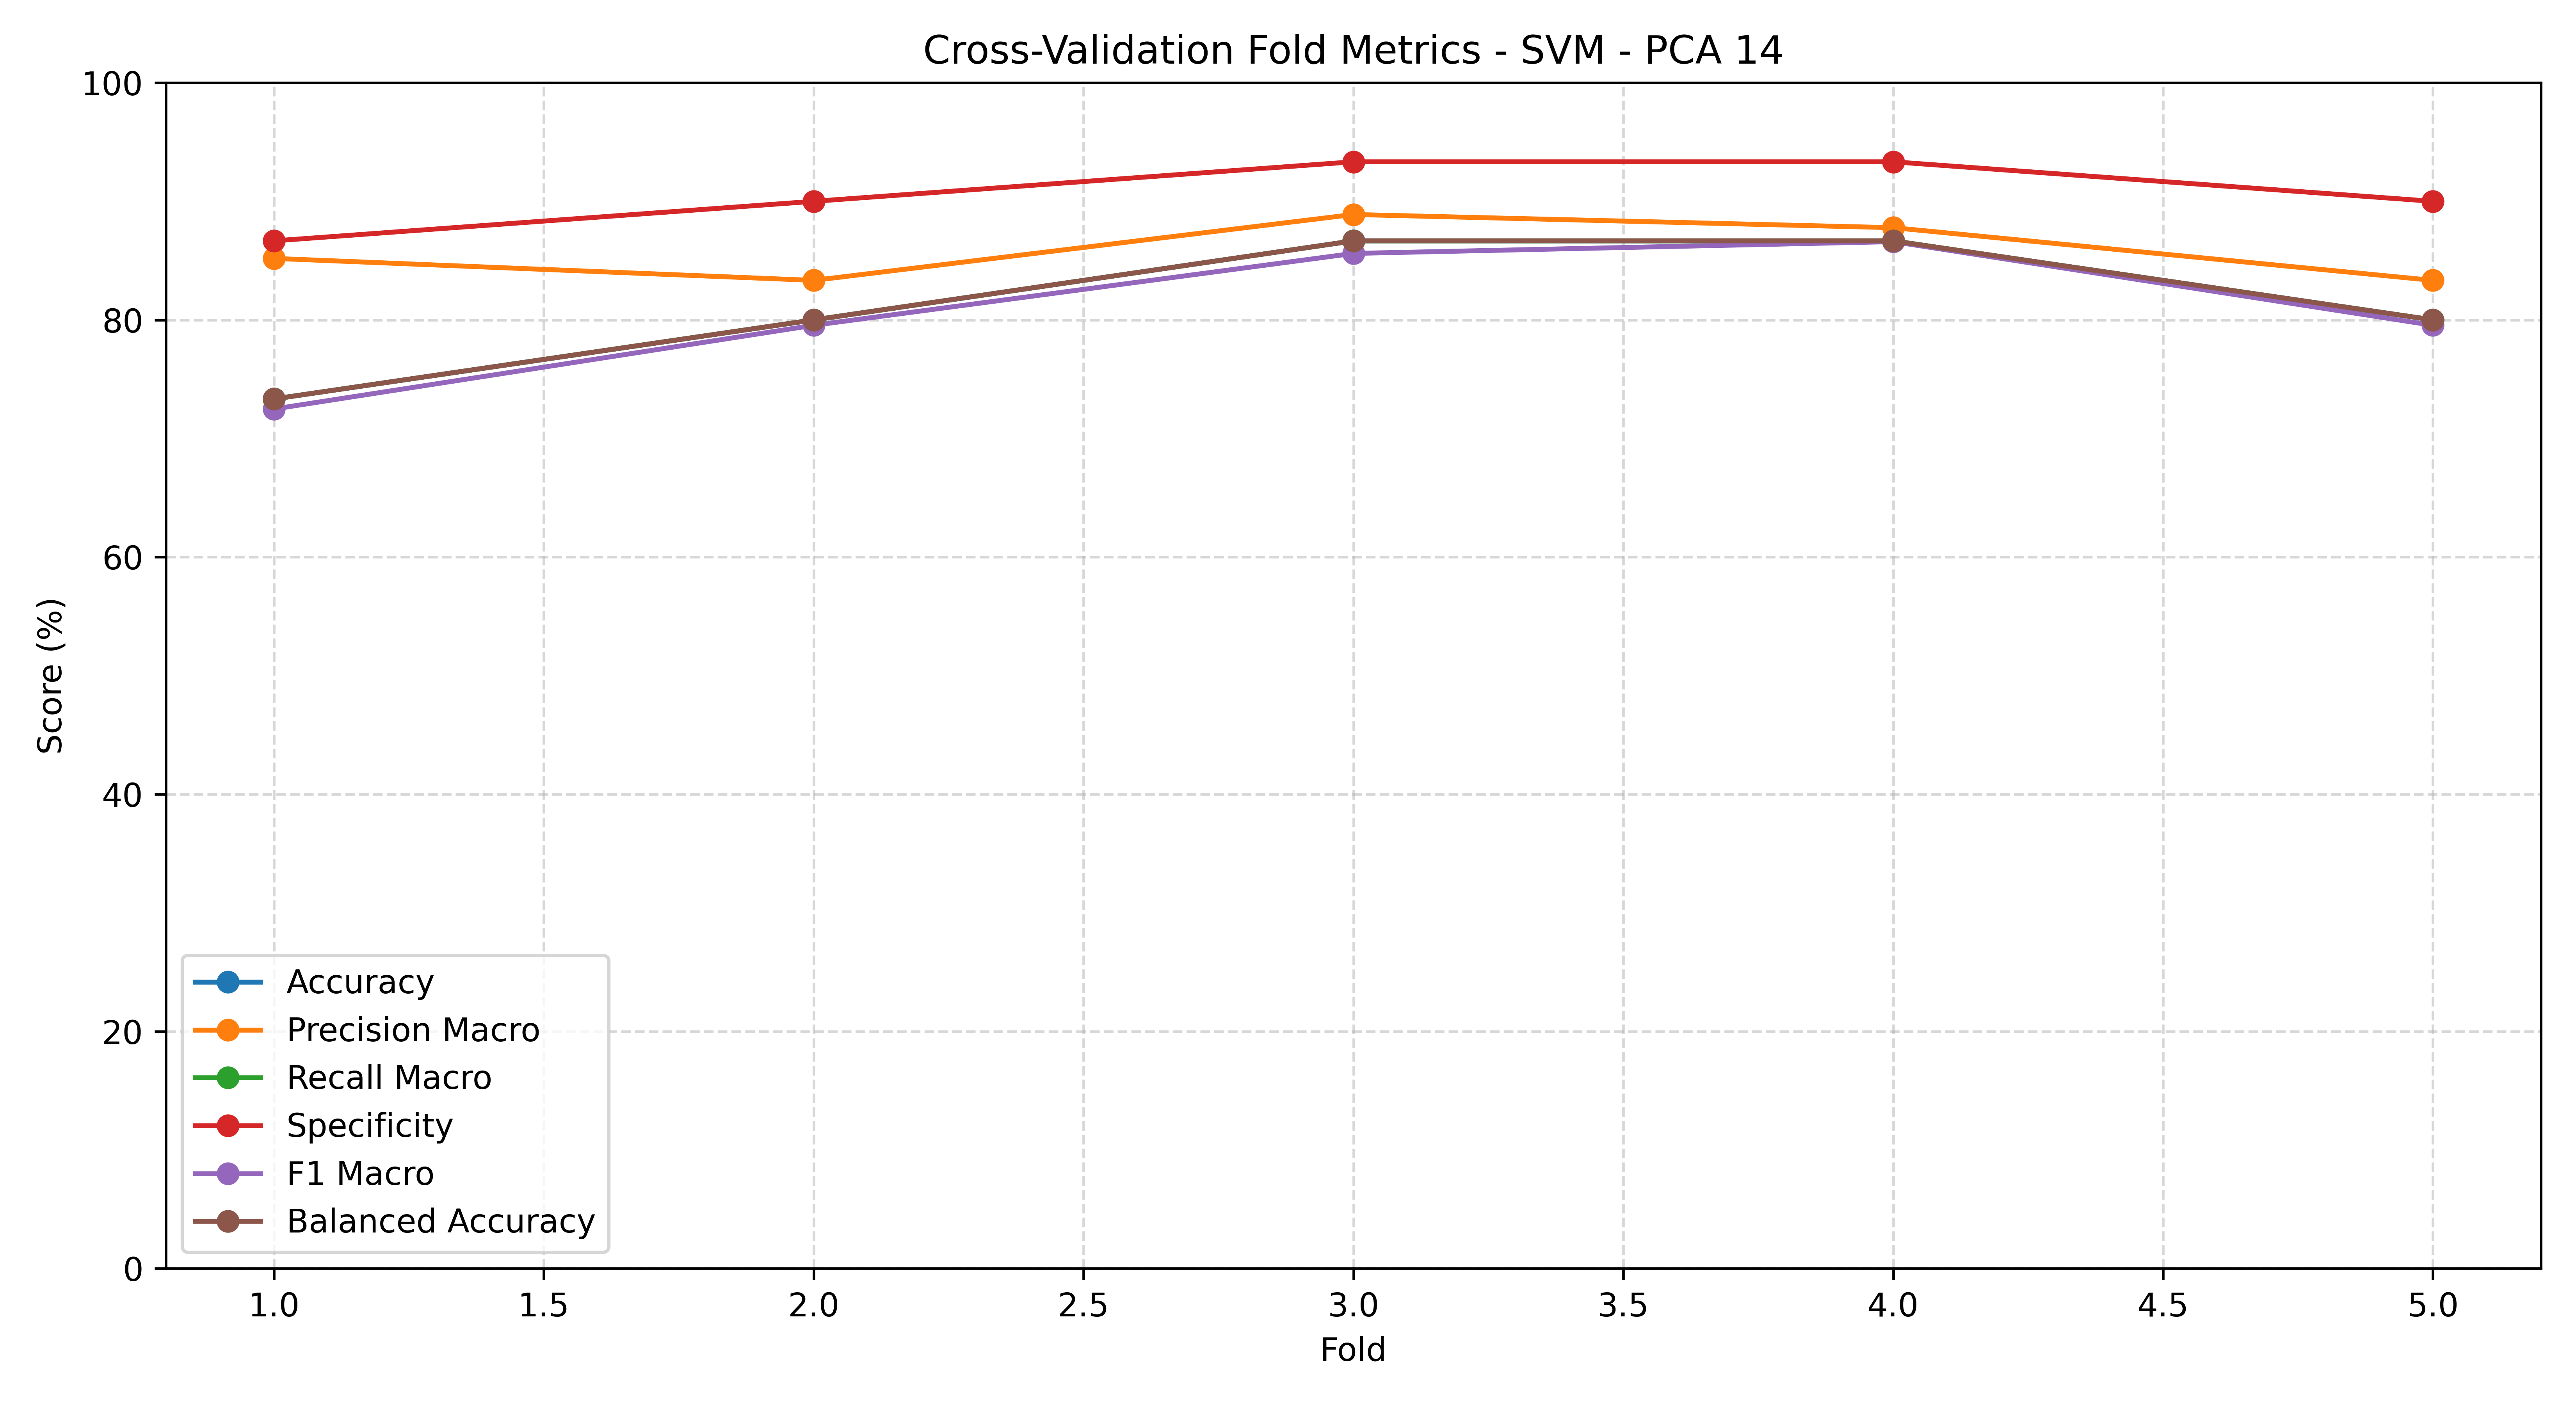
\includegraphics[width=0.8\linewidth]{../Results/Sit_To_Stand/Final/Final_Model_SVM_PCA14/Figures/CV_Fold_Metrics}
	\caption{نتایج ارزیابی مدل منتخب برای فعالیت برخاستن از زمین در تقسیم‌بندی‌های مختلف}
	\label{fig:Sit_To_Stand_cv_fold_metrics}
\end{figure}

برای بررسی نوع خطاهای مدل، ماتریس درهم‌ریختگی نرمال‌شده در
\autoref{fig:Sit_To_Stand_normalized_confusion_matrix}
ارائه شده است.

\textbf{TODO: مشخص شود کدام طبقه با دقت بیشتری تشخیص داده شده و بیشترین اشتباه میان کدام دو سطح عملکردی رخ داده است. در صورت وجود خطای بیشتر میان طبقه‌های مجاور، به شباهت الگوهای حرکتی آن‌ها اشاره شود.}

\begin{figure}[H]
	\centering
	
\includegraphics[width=0.6\linewidth]{../Results/Sit_To_Stand/Final/Figures/Normalized_Confusion_Matrix}
	\caption{ماتریس درهم‌ریختگی مدل منتخب برای فعالیت برخاستن از زمین}
	\label{fig:Sit_To_Stand_normalized_confusion_matrix}
\end{figure}

در مجموع، نتایج این فعالیت نشان می‌دهند که تحلیل هم‌زمان اطلاعات حسگرهای نصب‌شده روی سر، دست‌ها و پاها می‌تواند تفاوت موجود میان راهبردهای مختلف برخاستن از زمین را آشکار کند. کاهش بعد ویژگی‌ها نیز با حذف اطلاعات همبسته و کاهش پیچیدگی مدل، امکان دستیابی به یک ساختار مناسب‌تر برای طبقه‌بندی سطوح عملکردی را فراهم کرده است.
